% Preamble for the typeset manuscript. The body is generated from
% paper/manuscript.md by paper/build.py -- do not edit manuscript.tex by hand.
%
% manuscript.md is the single source of truth: tests/test_canonical_numbers.py
% asserts it against results/canonical_numbers.json. An earlier round of this
% project shipped two artifacts written by different runs that disagreed in the
% third decimal; keeping a hand-maintained .tex alongside the .md would be the
% same mistake in a different place.

\documentclass[11pt]{article}

\usepackage[margin=1in]{geometry}
\usepackage{amsmath}
\usepackage{amssymb}
\usepackage{booktabs}
\usepackage{longtable}
\usepackage{graphicx}
\usepackage{array}
\usepackage{calc}
\usepackage{caption}
\usepackage{microtype}
\usepackage[hidelinks]{hyperref}
\usepackage{newunicodechar}

\graphicspath{{../results/figures/}}

\captionsetup{font=small,labelfont=bf}
\setlength{\tabcolsep}{5pt}
\renewcommand{\arraystretch}{1.15}
\setlength{\emergencystretch}{3em}
% The markdown headings already carry their own numbers ("4.1 Omega fails"),
% so LaTeX must not add a second set on top of them.
\setcounter{secnumdepth}{0}
\urlstyle{same}

% pandoc emits these
\providecommand{\tightlist}{%
  \setlength{\itemsep}{0pt}\setlength{\parskip}{0pt}}
\providecommand{\pandocbounded}[1]{#1}
% pandoc wraps uncaptioned longtables in \def\LTcaptype{none}; longtable then
% steps a counter of that name, which does not otherwise exist.
\newcounter{none}

% The manuscript's non-ASCII characters, mapped so the document builds with
% ordinary Computer Modern rather than depending on a system Unicode font.
\newunicodechar{Ω}{\ensuremath{\Omega}}
\newunicodechar{α}{\ensuremath{\alpha}}
\newunicodechar{×}{\ensuremath{\times}}
\newunicodechar{−}{\ensuremath{-}}
\newunicodechar{≥}{\ensuremath{\ge}}
\newunicodechar{≈}{\ensuremath{\approx}}
\newunicodechar{→}{\ensuremath{\rightarrow}}
\newunicodechar{↔}{\ensuremath{\leftrightarrow}}
\newunicodechar{₀}{\ensuremath{_0}}
\newunicodechar{₂}{\ensuremath{_2}}
\newunicodechar{₅}{\ensuremath{_5}}
\newunicodechar{⁻}{\ensuremath{^-}}
\newunicodechar{⁵}{\ensuremath{^5}}
\newunicodechar{⁷}{\ensuremath{^7}}
\newunicodechar{é}{\'e}

\title{Calibration and evaluation of disproportionality nulls for drug--drug interaction detection: an analysis of 22 years of FAERS}
\author{[TODO: author list and affiliations]}
\date{\today}

\begin{document}
\maketitle

\begin{abstract}

\textbf{Background.} Drug--drug interactions (DDIs) are largely identified after
approval, and spontaneous reporting databases are the primary instrument. The
established disproportionality measure for DDI surveillance, Ω (Norén et al.,
2008), uses a null in which the joint relative risk of two drugs is the product
of their individual relative risks. Whether that null is appropriate for an
adverse event whose leading reported causes are the drugs being tested has not,
to our knowledge, been examined empirically.

\textbf{Methods.} We assembled the complete public history of the FDA Adverse Event
Reporting System --- 90 quarterly archives, 2004Q1--2026Q2, 328,476,258 rows ---
and reduced it to 20,293,421 distinct cases by six-stage deduplication including
a cross-era identifier bridge validated against a chance baseline. After
excluding 19,005 cases listing more than 20 drugs (see Results), the analysis
population was \textbf{20,274,416 cases carrying 41,889 myotoxicity events (0.207\%)}.
Drug entries were resolved to active ingredients (98.0\% of 73.96M rows) and the
event was defined by 23 hand-curated MedDRA Preferred Terms in 10 concepts,
verified continuous across two MedDRA renamings. We validated against 16
positive controls, measured the false-positive rate against the full pool of
16,138 generated negative controls, and screened 17,375 drug pairs.

\textbf{Deviation from protocol.} Ω was pre-specified and \textbf{failed}, recovering
4/16 positive controls against \textbf{12/16} for an additive (excess-risk) null at
the same threshold. The pooled false-positive rates of the two nulls are close
(6.4\% vs 6.7\%), but that pooling is over a pool that does not occupy the regime
where recovery is measured; in regime the rates are 2.2\% (95\% CI 1.24--3.34\%,
cluster bootstrap over drugs) and 9.3\% (7.29--11.32\%), so the
recovery comparison is between two very different operating points (§4.6).
We adopted the additive null after observing this. Ω also becomes more negative
as the marginal associations strengthen (r = −0.63, n = 16, 95\% CI −0.86 to
−0.19, p = 0.009) --- but so does Ω\_add (r = −0.65, p = 0.007), while the
\emph{observed} joint event rate rises far more shallowly with marginal strength
than either null predicts (r = +0.12, 95\% CI −0.40 to +0.58).
Both nulls therefore over-predict for strongly-associated pairs; what separates
them is the size of the expectation, not its gradient. Because the estimand was
selected on the evaluation set, the (binary) selection was cross-validated: the
additive null wins in \textbf{16/16 leave-one-out folds}. Stable selection forces
leave-one-out recovery to equal in-sample recovery, so the reported optimism of
0.000 is a consequence of that stability rather than independent evidence, and
it does not address the choice of controls (§4.10). Both measures are reported
throughout.

\textbf{Results.} Under the additive null the pipeline recovered \textbf{12/16} controls
(12/14 adequately powered; 95\% CI \textbf{50--100\%}, resampling the victim drug, since
the 16 controls are five victim drugs and simvastatin appears in seven) against
4/16 for Ω at the same threshold. Two binary design choices were available --- event
tier and drug role policy --- and all four arms are reported: the additive
advantage holds in three (+8, +8, +7 pairs) and is \textbf{null in the fourth}
(broad tier with the wider role policy, 6/16 against 6/16). On a second control set selected by FDA labelling rather than by the
authors (349 pairs), the same direction holds at both operating points ---
additive 55 vs multiplicative 29 at Ω₀₂₅ \textgreater{} 0, and 42 vs 15 at the calibrated
threshold --- but the recovery \textbf{rate falls to 12--16\%}. That gap is not power:
recovery \emph{falls} as co-reporting rises, because the most heavily co-reported
label-documented pairs show event rates at or below the database baseline and
carry class rather than pair-specific warnings. \textbf{Neither 86\% nor 12\% is the
sensitivity of the method}; they bracket it. The failure of Ω replicates on an
independent drug-dominant event matched on event rate, torsade de pointes
(\textbf{0/10} multiplicative vs 9/10 additive). The false-positive rate at Ω₀₂₅ \textgreater{} 0
was 6.7\% against a nominal 2.5\% (multiplicative 6.4\%); the threshold was
calibrated to Ω\_add,025 \textgreater{} +0.436 and validated out of sample at
\textbf{5.03\% (95\% CI 4.37--5.74\%)}. The screen returned 1,022 signals of which
\textbf{874 (759--997)} are expected by chance; Benjamini--Hochberg at q = 0.05 on
Poisson tail probabilities returns 1,147, so the shrinkage rule is the more
conservative of the two.

\textbf{The screen shows no enrichment for genuine interactions once the annotation is made independent of the control set.}
Pooled enrichment of known interaction pairs appears significant (2.02×, 95\% CI
1.59--2.55), but every positive-control drug is also on the list defining ``known
pair'', so the annotation is not independent of the control set. Restricting to
pairs containing \textbf{no} positive-control drug, enrichment is \textbf{1.12× (95\% CI
0.69--1.81)} --- indistinguishable from unity. This is confirmed against an \textbf{independent,
endpoint-specific reference built from FDA product labelling} (709 pairs in
which one drug's label names the other within 600 characters of a myotoxicity
term, capturing 16/16 positive controls): enrichment 3.52×
(2.71--4.56) over all pairs, falling to \textbf{1.23× (0.67--2.24)} once
control drugs are excluded, and to \textbf{1.045} after stratifying on co-report
count. The band in which a novel
interaction would appear shows enrichment \textbf{below} unity (0.77×, 95\% CI
0.66--0.89). The reference is also structurally blind to 9.9\% of screened
pairs --- 11 of the 200 screened ingredients (5.5\%) have no FDA label at all,
among them fusidic acid --- and restricting to pairs whose two labels both
exist leaves enrichment at \textbf{1.067 (0.292--1.972)}, unchanged. Requiring the
signal to persist independently in all three eras yields 19 pairs, but the same
filter applied to negative controls admits 0.093\% of them (95\% CI
0.039--0.191\%), implying \textbf{16.1 era-stable pairs by chance (95\% CI 6.7--33.2)
against 19 observed}; and under the endpoint-specific reference with control
drugs removed, \textbf{none} of the 19 is documented. Neither how many pairs survive
the filter nor which ones is distinguishable from the null.

\textbf{Conclusions.} We report a validated pipeline, a characterised false-positive
rate, and a negative discovery result. The robust methodological finding is that
the multiplicative null is unusable for events where the drugs of interest are
the dominant reported cause --- demonstrated on two such events. Whether that
condition is what \emph{causes} the failure remains a hypothesis: we could not
assemble an adequately powered event with weak marginals to serve as the
negative case. The negative discovery result is bounded by the reference rather
than by the method: the screen's highest-ranked pair by event rate,
atorvastatin + fusidic acid (155 events in 185 co-reports), is a contraindicated
interaction that \textbf{no} reference available to us contained. A secondary finding is that 0.09\% of
reports --- those listing more than 20 drugs --- contribute 34.7\% of all drug pairs
at a 4× enriched event rate, and must be capped in any pairwise screen. Claims
that this class of screen discovers novel interactions should be treated with
scepticism until the annotation used to evaluate them is independent of the
control set used to build them.

\begin{center}\rule{0.5\linewidth}{0.5pt}\end{center}

\end{abstract}

\section{1. Introduction}\label{introduction}

Most drug--drug interactions are discovered after approval. Pre-marketing trials
cannot test the combinatorial space, so post-marketing surveillance of
spontaneous reports carries the burden. FAERS is the largest public instrument
for this in the United States.

Rhabdomyolysis is a natural target: severe, with well-characterised drug causes
and an unusually strong positive-control set in the statin interactions. That
same property --- the controls being the dominant causes of the outcome --- creates
the methodological problem which is this paper's main contribution.

We set out to (i) build a reproducible pipeline over the complete FAERS history,
(ii) validate it against known interactions, (iii) measure its false-positive
rate, and (iv) screen for undocumented interactions. Aims (i)--(iii) succeeded.
Aim (iv) returned a negative result, which we report as the finding.

\section{2. Related work}\label{related-work}

\begin{quote}
\textbf{Verification status.} Every citation below has been verified against an
indexed source; full bibliographic detail is in §8. One exception is recorded
explicitly: the Ω definition used here (α = 0.5, threshold Ω₀₂₅ \textgreater{} 0) is
corroborated by two independent \emph{secondary} sources --- a peer-reviewed review
of DDI signal-detection methods stating that ``α = 0.5 was set to provide
sufficient shrinkage for avoiding disproportional highlighting based on rare
reports'', and the Uppsala Monitoring Centre's operational documentation
listing ``Interaction disproportionality measure Omega 025 \textgreater{} 0'' --- but \textbf{the
primary paper is paywalled and has not been read by the authors.} A single
further work on FAERS duplication practice was cited in an earlier draft and
has been removed rather than cited from memory, as its bibliographic detail
could not be confirmed.
\end{quote}

\textbf{Disproportionality for single drug--event pairs.} The standard measures are
the proportional reporting ratio (Evans, Waller and Davis, 2001), the Bayesian confidence propagation neural network / information
component (Bate et al., 1998), and
the multi-item gamma-Poisson shrinker (DuMouchel, 1999). All share the shrinkage logic used here: a lower credibility
bound withholds a signal at low counts.

\textbf{Extension to drug pairs.} Thakrar, Grundschober and Doessegger (2007) set out additive and multiplicative models for interaction
signals in spontaneous reports and noted that the two answer different
questions. Norén, Sundberg, Bate and Edwards (2008)
introduced Ω, the measure this study pre-specified, comparing the observed triple count against
a log-linear model with all pairwise associations and no three-way term.
Our contribution is not a new estimator but an empirical demonstration of where
Ω's null breaks down, and the identification of the condition under which it
does.

\textbf{Additive versus multiplicative interaction.} The argument that departure from
\emph{additivity} is the criterion for interaction of public-health relevance, while
departure from multiplicativity answers a different question, is long-standing
in epidemiology (Rothman, 1976), where departure from additivity is the test for synergism
under the sufficient-cause framework. VanderWeele and Knol (2014) give the
modern treatment, and their recommendation --- that both scales be reported rather
than one chosen --- is the practice adopted here. We rediscovered
this argument empirically and then found it already established; we claim
novelty only for the demonstration in the spontaneous-reporting setting.

\textbf{FAERS curation.} Banda et al.~(2016) published AEOLUS, a curated
and standardised FAERS resource covering January 2004 to June 2015, retaining
4,928,413 unique cases. Over the identical window this pipeline retains
5,337,888 --- a difference of 8\%, in the direction expected given that AEOLUS
applies an additional pass deduplicating on event date, age, sex and country
alone regardless of case number (§6). The DiAna dictionary (Fusaroli et al., 2024) provides a
curated FAERS drugname→ingredient mapping. We did not use it, having found that
FDA's own \texttt{prod\_ai} field applied backwards suffices --- and the two agree closely
on coverage: DiAna reports standardising \textbf{98.94\%} of 74,143,411 drug entries;
this pipeline resolves \textbf{98.0\%} of 73,960,283. That near-agreement, reached by
independent means, is the closest thing to an external check on the ingredient
resolution available here.

\textbf{DDI reference sets.} TWOSIDES (Tatonetti et al., 2012) is derived from FAERS itself and is therefore unsuitable as an
independent reference here. DrugBank is licensed and was not available.

The ONC high-priority DDI list (Phansalkar et al., 2012) \emph{is} available --- it is
a 15-row table in an open-access paper, and an earlier draft of this manuscript
described it as unavailable without checking. It was retrieved and examined. It
is \textbf{not usable as a reference for this study}, for a reason specific to it
rather than to access: the list is expressed as \emph{drug-class} pairs (for example
``HMG Co-A reductase inhibitors ↔ CYP3A4 inhibitors'', ``QT prolonging agents ↔ QT
prolonging agents''), not as ingredient pairs, so applying it requires an
ingredient→class mapping that would itself have to be author-written --- the
circularity this study is trying to escape. Only one of the 15 concerns
myotoxicity, and the paper explicitly \emph{excluded} the gemfibrozil--statin
interaction, one of this study's positive controls, on the grounds that ``clinical
benefit of co-prescribing outweighs risk''. A 15-row class-level list that
excludes the canonical myotoxicity pair cannot serve as the endpoint-specific
reference this evaluation needs.

\textbf{A curated, ingredient-level, severity-graded DDI compendium remains
unavailable, and that is the single largest limitation of the evaluation} (§6).

\section{3. Methods}\label{methods}

\section{3.1 Data acquisition}\label{data-acquisition}

All 90 quarterly archives (3.55 GB compressed, 20.04 GB uncompressed) were
downloaded with a manifest recording a SHA-256 per archive, since FDA silently
re-issues quarterly files.

The archives are not one format. An audit of every column header in every table
across all 90 quarters found 21 schema changepoints, three of which would have
corrupted results without raising an error:

\begin{itemize}
\tightlist
\item
  \textbf{A UTF-8 byte-order mark} on the first column name of \texttt{DRUG12Q4.txt} and
  nowhere else, so every drug-to-demographics join for that quarter matches zero
  rows.
\item
  \textbf{2012Q4 spells three columns differently from both neighbours}
  (\texttt{outc\_code}/\texttt{outc\_cod}, \texttt{lot\_nbr}/\texttt{lot\_num}, \texttt{i\_f\_code}/\texttt{i\_f\_cod}).
\item
  \textbf{\texttt{DEMO18Q1\_new.txt}} --- a non-standard filename that a pattern anchored on
  \texttt{Q\textless{}digit\textgreater{}.TXT} classifies as documentation, silently dropping a quarter of
  demographics.
\end{itemize}

Deleted-case lists ship for 2019Q1--2026Q2 under five naming conventions,
including \texttt{Deleted/DELETEnnQn.txt} from 2021Q4, which contains no occurrence of
``deleted''. A cumulative list in 2019Q1 covers everything prior.

\section{3.2 Parsing}\label{parsing}

Every data line in every FAERS table ends with a trailing delimiter its header
does not declare. Given more fields than names, pandas promotes the surplus
leading column to the index and shifts every column left by one, silently. In
\texttt{DRUG} this moves \texttt{drug\_seq} into \texttt{primaryid}; both are integers, every type
check passes, and the pipeline completes with every drug attributed to the wrong
report. Parsing is therefore validated by referential integrity rather than by
type: \textbf{0 orphans across all 328,476,258 rows}.

\section{3.3 Deduplication}\label{deduplication}

Six stages, 24,812,425 raw demographics rows → 20,293,421 distinct cases.
\textbf{The first two rows are per-era, not cumulative}: LAERS and FAERS use disjoint
identifier spaces and are deduplicated separately before being bridged, so their
\texttt{remaining} values are counts within their own era (4,276,201 and 20,536,224 raw
rows respectively) and sum to 20,775,025 entering the bridge. Rows from the
cross-era bridge down are cumulative. Seven LAERS rows carry a NULL \texttt{case\_id}
and are dropped before stage 1, so the two era totals sum to 24,812,418 rather
than the 24,812,425 raw.

{\def\LTcaptype{none} % do not increment counter
\begin{longtable}[]{@{}
  >{\raggedright\arraybackslash}p{(\linewidth - 4\tabcolsep) * \real{0.2727}}
  >{\raggedleft\arraybackslash}p{(\linewidth - 4\tabcolsep) * \real{0.3636}}
  >{\raggedleft\arraybackslash}p{(\linewidth - 4\tabcolsep) * \real{0.3636}}@{}}
\toprule\noalign{}
\begin{minipage}[b]{\linewidth}\raggedright
stage
\end{minipage} & \begin{minipage}[b]{\linewidth}\raggedleft
remaining
\end{minipage} & \begin{minipage}[b]{\linewidth}\raggedleft
removed
\end{minipage} \\
\midrule\noalign{}
\endhead
\bottomrule\noalign{}
\endlastfoot
raw DEMO rows (all eras) & 24,812,425 & --- \\
within-LAERS, per era (highest \texttt{isr} per case) & 3,091,161 & 1,185,033 \\
within-FAERS, per era (highest \texttt{caseversion}) & 17,683,864 & 2,852,360 \\
cross-era bridge & 20,692,683 & 82,342 \\
FDA-deleted cases & 20,588,497 & 104,186 \\
near-duplicates & 20,294,190 & 294,307 \\
one case per report & 20,293,421 & 769 \\
\end{longtable}
}

\textbf{The cross-era bridge was validated, not assumed.} 82,342 identifiers appear
in both numbering systems. Event date agreed on 33.3\% of them against 0.0\% at a
chance baseline; all of date/sex/age on 26.0\% against 0.0\%.

Near-duplicate eligibility requires event date, age, drug set and PT set rather
than a count of populated fields; an initial ``any 4 of 6'' rule removed 14.5\% of
all cases with a largest group of 9,270, a collision among sparse records.

\section{3.4 Ingredient resolution}\label{ingredient-resolution}

\texttt{prod\_ai} exists only from 2014Q3 (97.8\% coverage after, 0\% before). The modern
era was used as an FDA-curated \texttt{drugname\ →\ ingredient} lookup and applied
backwards, resolving 90.1\% of LAERS rows; a relaxed pass stripping dose and
packaging detail added \textasciitilde6 points, for \textbf{98.0\% of 73,960,283 rows}. Salt and
hydrate forms are stripped; element-headed compounds (calcium carbonate, ferrous
sulfate) are protected.

\textbf{Coverage is not accuracy.} No manual validation of resolution correctness was
performed; see §6.

\section{3.5 Event definition}\label{event-definition}

23 PTs in 10 concepts, curated against the 25,047 PT strings actually present
rather than a current MedDRA release. Two renamings occur within the concept
area, both clean instantaneous switches: \texttt{BLOOD\ CREATINE\ PHOSPHOKINASE\ INCREASED} → \texttt{CREATINE\ KINASE\ INCREASED} at 2026Q2 (part of a vocabulary-wide
event in which 1,907 PT strings make their last appearance in 2026Q1), and
\texttt{IMMUNE-MEDIATED\ NECROTISING\ MYOPATHY} → \texttt{IMMUNE-MEDIATED\ MYOSITIS} at 2019Q4.
The latter is \emph{not} meaning-preserving --- the successor carries \textasciitilde5× the
per-quarter volume --- so both are held out of the primary tier.

\section{3.6 The positive control set, and its verification}\label{the-positive-control-set-and-its-verification}

16 pairs, assembled from FDA product labelling: seven simvastatin pairs, two
lovastatin, two atorvastatin, two rosuvastatin and three colchicine, against
eight perpetrator drugs.

\textbf{Every pair was checked against label text rather than asserted.} An earlier
version of this work carried \texttt{citation\_status:\ to\_verify} on all sixteen rows of
the control file --- a field created with the intention of checking them, never
filled in --- while §2 interrogated the \emph{evaluation} reference at length. The
check (\texttt{faers\_ddi.verify\_controls}, run against the same cached label corpus as
§3.7) asks whether either drug's label names the other, whether a myotoxicity
term appears within 600 characters of that mention, and whether the mention sits
in contraindication or dose-limiting language:

{\def\LTcaptype{none} % do not increment counter
\begin{longtable}[]{@{}
  >{\raggedright\arraybackslash}p{(\linewidth - 2\tabcolsep) * \real{0.4286}}
  >{\raggedleft\arraybackslash}p{(\linewidth - 2\tabcolsep) * \real{0.5714}}@{}}
\toprule\noalign{}
\begin{minipage}[b]{\linewidth}\raggedright
status
\end{minipage} & \begin{minipage}[b]{\linewidth}\raggedleft
pairs
\end{minipage} \\
\midrule\noalign{}
\endhead
\bottomrule\noalign{}
\endlastfoot
named, myotoxicity-relevant, \textbf{and contraindicated or dose-limited} & \textbf{14} \\
named and myotoxicity-relevant & 2 \\
named only, or not found & 0 \\
\end{longtable}
}

All 16 are confirmed. Two --- colchicine + cyclosporine and colchicine +
atorvastatin --- carry a myotoxicity warning without explicit dose restriction,
and colchicine + atorvastatin is additionally the one pair sourced from case
reports rather than labelling and graded \texttt{probable} rather than \texttt{established}.
It is retained and flagged rather than dropped: removing a control because it
scored poorly would be selection on the evaluation set.

\textbf{The 16 are not 16 independent trials.} They are five victim drugs, and
simvastatin appears in seven of them. Recovery intervals are therefore computed
by resampling the victim drug (§4.3), not by a binomial on the pair count.

\section{3.7 Independent interaction reference}\label{independent-interaction-reference}

Because the authors wrote both the positive control set and the list defining
``known pair'', a second annotation was built that they did not author. Signals
are evaluated against \textbf{three annotations} of increasing independence --- the
authors' own curated list, FDA labelling for any endpoint, and FDA labelling
restricted to this endpoint --- each applied both to all pairs and to pairs
containing no positive-control drug. For each
of the 200 screened ingredients we retrieved the most recent FDA product label
via openFDA and recorded which other screened ingredients are named in its DRUG
INTERACTIONS, CONTRAINDICATIONS or WARNINGS AND PRECAUTIONS sections. A pair is
\texttt{label\_documented} when either drug's label names the other. Labels are cached
so the reference is fixed against future label revisions.

\textbf{This is independent of the authors but not of FAERS.} Labelling is informed
by post-marketing surveillance, so it cannot establish that a signal was found
independently of the data; it establishes only that the annotation was not
written by us, which is the circularity at issue. Labels also warn by class
(``strong CYP3A4 inhibitors'') as often as by name, so the reference is
under-sensitive, biasing measured enrichment downward.

\textbf{That is the conservative direction for a claim that enrichment exists, and the
anti-conservative direction for this paper's actual claim, which is that it does
not.} Attenuating a ratio toward unity moves it toward our own conclusion, so
under-sensitivity cannot be offered as a safeguard here. §4.5 therefore reports
the analysis restricted to pairs whose two labels both exist, which removes the
part of the insensitivity that is structural rather than editorial.

\section{3.8 Statistical measures}\label{statistical-measures}

The eight cells of the 2×2×2 table are recoverable from the triple count, six
marginals and the total.

Write \(n_{111}\) for the count of cases reporting drug \(A\), drug \(B\) and event
\(Z\); \(n_{11\cdot}\) for the co-report count; \(p_A = P(Z \mid A)\),
\(p_B = P(Z \mid B)\) and \(p = P(Z)\) for the two marginal risks and the database
background; and \(\alpha\) for the shrinkage constant. Both statistics compare
\(n_{111}\) against an expectation and differ \textbf{only} in how that expectation is
formed.

\textbf{Ω (multiplicative null).} The expectation \(E^{\mathrm{mult}}_{111}\) is the
fit of the log-linear model \([AB][AZ][BZ]\) --- all pairwise associations, no
three-way term:

\[\Omega = \log_2\!\left(\frac{n_{111} + \alpha}{E^{\mathrm{mult}}_{111} + \alpha}\right)\]

fitted exactly by iterative proportional fitting rather than the published
closed-form approximation, which we measured at up to 237\% error once pairwise
log-odds reach 2 --- enough to produce Ω \textless{} −1 on tables with no synergy.

\textbf{Ω\_add (additive null), primary.} The expectation is the joint risk under
additivity of excess risk, floored at the larger single-drug risk and capped at
1, applied to the co-report count:

\[E^{\mathrm{add}}_{111} = n_{11\cdot}\,\min\!\big(\max(p_A + p_B - p,\; p_A,\; p_B),\;1\big)\]

\[\Omega_{\mathrm{add}} = \log_2\!\left(\frac{n_{111} + \alpha}{E^{\mathrm{add}}_{111} + \alpha}\right)\]

The floor is not at zero: when both drugs are reported with the event \emph{less}
often than background, \(p_A + p_B - p < 0\), and clipping to zero would make the
expected count zero and Ω\_add unbounded in the observed count. The cap at 1
binds precisely in the drug-dominant regime this paper is about, where
\(p_A + p_B\) can exceed unity. Shrinkage is identical for both, so the two
estimands differ only in the null.

\(\Omega_{025}\) and \(\Omega_{\mathrm{add},025}\) denote the 2.5th percentile of
the corresponding gamma-Poisson posterior.

\textbf{Shrinkage constant.} α = 0.5 is conventional and could not be verified
against Norén et al.~It is therefore varied across a 20-fold range as a
sensitivity analysis (§4.8) rather than assumed.

\textbf{Intervals and tests.} All proportions carry Jeffreys 95\% intervals; ratios
carry log-scale intervals. Binomial tests are \textbf{not} used for inference:
with 200 drugs each drug sits in 199 pairs, so pair outcomes are strongly
dependent. Significance is assessed by a permutation test that holds the pair
graph and the observed signal pattern fixed and randomises which drugs are
annotated as implicated (10,000 permutations).

\textbf{What ``nominal 2.5\%'' does and does not mean.} Ω₀₂₅ is the 2.5th percentile of
a gamma-Poisson posterior rather than a frequentist test statistic, so ``nominal
2.5\%'' is a convention of the field and not a guarantee of the estimator; a rate
departing from it is evidence about behaviour in this regime, not a violated
guarantee. We use the convention because it is the operating point
practitioners use, and because the comparisons below hold the cut fixed across
both measures.

\textbf{Design.} Unit of analysis is the case; denominator is the deduplicated set
less the polypharmacy exclusion, retaining cases with no resolved drug as
background; drug roles are primary/secondary suspect plus interacting.

\section{4. Results}\label{results}

\section{4.1 Ω fails; both nulls mispredict in the same direction (Figures 1--2)}\label{ux3c9-fails-both-nulls-mispredict-in-the-same-direction-figures-12}

Ω recovered \textbf{4/16} positive controls at Ω₀₂₅ \textgreater{} 0, against \textbf{12/16} for the
additive null at the same threshold. Pooled over the generated negative controls
the two nulls' false-positive rates are 6.4\% and 6.7\%. \textbf{Those pooled rates do
not describe the regime in which the recovery comparison is made}, and an
earlier version of this manuscript presented them as though they did, calling
the comparison matched. §4.3 shows they do not: among pairs as strongly
associated as the positive controls the rates are 2.2\% and 9.3\%, and once they
are equalised the recovery gap falls from eight pairs to one or two.

Simvastatin + amiodarone, named in advance as the pair that must work, scored
Ω = \textbf{−0.385} (Ω₀₂₅ = −0.630): 145 events among 649 co-reports against 189.5
expected under the multiplicative null.

The drugs of interest are the dominant reported causes of the outcome, with
marginal relative risks of 3--19 against a 0.207\% background, so the
multiplicative null predicts very high joint rates (Figure 1):

{\def\LTcaptype{none} % do not increment counter
\begin{longtable}[]{@{}lrrr@{}}
\toprule\noalign{}
pair & observed & multiplicative & additive \\
\midrule\noalign{}
\endhead
\bottomrule\noalign{}
\endlastfoot
gemfibrozil + simvastatin & 56.2\% & 73.9\% & 28.3\% \\
atorvastatin + gemfibrozil & 14.9\% & 72.6\% & 23.1\% \\
amiodarone + simvastatin & 22.3\% & 29.2\% & 11.0\% \\
\end{longtable}
}

56\% of gemfibrozil + simvastatin co-reports carry rhabdomyolysis and the pair
still scores as protective.

\textbf{The marginal-strength gradient is real, but it is not diagnostic of the
multiplicative null.} Ω correlates with log₂(RR\_A × RR\_B) at
\textbf{r = −0.63 (n = 16, 95\% CI −0.86 to −0.19, p = 0.009)} (Figure 2). Because
Ω = log₂((O+α)/(E+α)) and E is an increasing function of the same marginals
that form the x-axis, part of any such correlation is induced by the
construction --- regressing a ratio on a proxy for its own denominator. We
measured how much: drawing the triple count from each null's own expectation and
recomputing the statistic 10,000 times gives an induced correlation centred on
zero (median +0.03, 95\% interval −0.23 to +0.26 for Ω). The observed −0.63 lies
outside that interval, so the gradient is \textbf{not} an artifact of the estimator.

It is, however, \textbf{not specific to the multiplicative null.} The additive null ---
this paper's remedy --- shows the same gradient, slightly stronger:

{\def\LTcaptype{none} % do not increment counter
\begin{longtable}[]{@{}
  >{\raggedright\arraybackslash}p{(\linewidth - 4\tabcolsep) * \real{0.3000}}
  >{\raggedright\arraybackslash}p{(\linewidth - 4\tabcolsep) * \real{0.3000}}
  >{\raggedleft\arraybackslash}p{(\linewidth - 4\tabcolsep) * \real{0.4000}}@{}}
\toprule\noalign{}
\begin{minipage}[b]{\linewidth}\raggedright
quantity regressed on log₂(RR\_A × RR\_B)
\end{minipage} & \begin{minipage}[b]{\linewidth}\raggedright
r (95\% CI)
\end{minipage} & \begin{minipage}[b]{\linewidth}\raggedleft
p
\end{minipage} \\
\midrule\noalign{}
\endhead
\bottomrule\noalign{}
\endlastfoot
\textbf{observed event rate among co-reports} & \textbf{+0.12 (−0.40 to +0.58)} & \textbf{0.67} \\
expected rate, multiplicative null & +0.94 & --- \\
expected rate, additive null & +0.94 & --- \\
Ω (multiplicative) & −0.63 (−0.86 to −0.19) & 0.009 \\
\textbf{Ω\_add (additive)} & \textbf{−0.65 (−0.86 to −0.22)} & \textbf{0.007} \\
\end{longtable}
}

\textbf{The observed joint event rate rises far more shallowly with marginal strength
than either null predicts.} The observed gradient is not distinguishable from
zero, but its interval (−0.40 to +0.58) admits a moderate rise, so the claim is
that the gradient is much shallower than predicted rather than that it is
absent. Both nulls predict a steep rise; both are therefore wrong in the
same direction, and the gradient in Ω reflects a property of the data --- joint
risk saturates as the individual risks grow --- rather than a defect peculiar to
multiplicativity. It will appear in any statistic that divides an observed rate
by a marginal-driven expectation.

\begin{quote}
An earlier version of this manuscript reported this correlation for Ω alone
and read it as evidence that the multiplicative null is uniquely broken. That
reading was incorrect. The correlation survives the artifact check, but it
does not separate the two nulls, and it is reported here for both.
\end{quote}

What \emph{does} separate them is \textbf{level, not slope}: the multiplicative
expectation is far larger at every point (72.9\% vs 27.9\% for gemfibrozil +
simvastatin), so the same saturation drives Ω below zero while leaving Ω\_add
above it. Departure from additivity is the standard criterion for clinically
meaningful interaction (Rothman, 1976; VanderWeele and Knol, 2014); departure
from multiplicativity is a stricter and different question, and on a
drug-dominant event it is a question almost nothing passes.

\section{4.2 The estimand switch does not inflate sensitivity}\label{the-estimand-switch-does-not-inflate-sensitivity}

The additive null was adopted because it recovered more controls, and control
recovery is then reported as validation --- selection on the evaluation set. The
selection decision is binary and was therefore cross-validated: the additive
null wins in \textbf{16/16 leave-one-out folds}, and held-out recovery equals
in-sample recovery (\textbf{12/16, optimism 0.000}).

\textbf{The optimism figure carries less information than it appears to.} When the
same null wins in every fold, the held-out score for each control is by
definition its in-sample score, so optimism is \emph{identically} zero --- it cannot
take another value. It is a consequence of the selection being stable, not
independent evidence for it, and an earlier version of this manuscript presented
it in the abstract as though it were a measurement. What leave-one-out does
establish is the stability itself: the choice between the two nulls does not
depend on any single control.

It does \textbf{not} address the deeper issue that these 16 controls were chosen by
the authors. That is addressed instead in §4.10, with a control set drawn by FDA
labelling rather than by us, and it is where the sensitivity estimate actually
degrades. See also §6.

\section{4.3 Tier A and Tier B}\label{tier-a-and-tier-b}

Under the additive null, \textbf{12/16 controls signal (12/14 powered)}, against
\textbf{4/16 for Ω (4/14 powered)} at the same threshold. Six of seven
simvastatin pairs and three of three colchicine pairs recover; both lovastatin
pairs have n\_ab of 13 and 1 and are unmeasurable. Both denominators are given
because they are not interchangeable: an earlier version quoted the additive
count out of 14 and the multiplicative count out of 16 in the same comparison.

\textbf{The interval must respect the control set's clustering.} The 16 controls are
five victim drugs and simvastatin appears in seven of them (§3.6), so they are
not 16 independent trials. Resampling the victim drug rather than the pair:

{\def\LTcaptype{none} % do not increment counter
\begin{longtable}[]{@{}lll@{}}
\toprule\noalign{}
estimate & naive binomial & \textbf{cluster bootstrap (victim drug)} \\
\midrule\noalign{}
\endhead
\bottomrule\noalign{}
\endlastfoot
12/14 powered = 86\% & 62--97\% & \textbf{50--100\%} \\
12/16 all = 75\% & 51--91\% & \textbf{30--96\%} \\
\end{longtable}
}

The naive interval is roughly 40\% too narrow. We report the clustered one. This
is the same correction already applied to the screen enrichment, where pairs
share drugs; applying it there and not here was two standards for one dependence
structure.

\textbf{The full specification grid.} Two binary design choices were available --- the
event tier (\texttt{core}, specific; \texttt{broad}, inclusive) and the drug role policy
(\texttt{primary}, suspect roles only; \texttt{sensitivity}, wider). \texttt{core}/\texttt{primary} is
pre-specified in \texttt{config.yaml} as \texttt{event.primary\_tier} and is the arm reported
throughout. All four were computed, and an earlier version of this manuscript
reported the pre-specified arm without disclosing that the others existed:

{\def\LTcaptype{none} % do not increment counter
\begin{longtable}[]{@{}
  >{\raggedright\arraybackslash}p{(\linewidth - 8\tabcolsep) * \real{0.1667}}
  >{\raggedright\arraybackslash}p{(\linewidth - 8\tabcolsep) * \real{0.1667}}
  >{\raggedleft\arraybackslash}p{(\linewidth - 8\tabcolsep) * \real{0.2222}}
  >{\raggedleft\arraybackslash}p{(\linewidth - 8\tabcolsep) * \real{0.2222}}
  >{\raggedleft\arraybackslash}p{(\linewidth - 8\tabcolsep) * \real{0.2222}}@{}}
\toprule\noalign{}
\begin{minipage}[b]{\linewidth}\raggedright
tier
\end{minipage} & \begin{minipage}[b]{\linewidth}\raggedright
role policy
\end{minipage} & \begin{minipage}[b]{\linewidth}\raggedleft
additive
\end{minipage} & \begin{minipage}[b]{\linewidth}\raggedleft
multiplicative
\end{minipage} & \begin{minipage}[b]{\linewidth}\raggedleft
additive advantage
\end{minipage} \\
\midrule\noalign{}
\endhead
\bottomrule\noalign{}
\endlastfoot
\textbf{core} & \textbf{primary} \emph{(pre-specified)} & \textbf{12/16} & \textbf{4/16} & \textbf{+8} \\
core & sensitivity & 12/16 & 4/16 & +8 \\
broad & primary & 11/16 & 4/16 & +7 \\
\textbf{broad} & \textbf{sensitivity} & \textbf{6/16} & \textbf{6/16} & \textbf{0} \\
\end{longtable}
}

\textbf{Under the widest event definition combined with the widest role policy, the
additive null's advantage disappears entirely.} The contrast holds in three of
four arms and is null in the fourth. Any reader weighing the headline result
should weigh that: it is robust to either widening alone, and not to both
together. The broad tier deliberately includes the two MedDRA concepts held out
of the primary definition for not being meaning-preserving (§3.5), and the
sensitivity policy admits concomitant drugs with no suspected causal role, so
the fourth arm is the least specific analysis available --- but it is not
unreasonable, and it is now on the record.

Against the \textbf{full pool of 16,138 negative controls} (not a sample --- sampling
2,000 left the threshold at the mercy of the draw, moving it by more than a
factor of four across legitimate runs), the pooled false-positive rates at
Ω₀₂₅ \textgreater{} 0 are \textbf{6.7\%} additive and \textbf{6.4\%} multiplicative, against a nominal
2.5\%. Reported by stratum, and for both nulls:

{\def\LTcaptype{none} % do not increment counter
\begin{longtable}[]{@{}lrrrr@{}}
\toprule\noalign{}
stratum & n & additive & multiplicative & ratio \\
\midrule\noalign{}
\endhead
\bottomrule\noalign{}
\endlastfoot
easy (neither drug RR ≥ 2) & 6,674 & 4.02\% & 4.94\% & 0.81 \\
hard (at least one RR ≥ 2) & 9,464 & 8.54\% & 7.50\% & 1.14 \\
\textbf{all} & 16,138 & \textbf{6.67\%} & \textbf{6.44\%} & 1.03 \\
\end{longtable}
}

An earlier version of this manuscript reported the strata for the additive null
alone and described the near-identical pooled rates as making the §4.1 recovery
comparison ``essentially matched''. \textbf{Both statements are withdrawn.} The pooled
figures are the average of two differences running in opposite directions, and ---
more importantly --- they are measured almost entirely outside the regime in which
recovery is measured.

\textbf{The negative and positive control populations barely overlap.} The generator
excludes any pair in which \emph{both} drugs are on the implicated list, a reasonable
guard against seeding the null set with true positives, but every positive
control is exactly such a pair --- so the generator \textbf{cannot produce a negative
that resembles a positive}, and that is a property of the exclusion rule
rather than of the data. Positive controls sit at a median
log₂(RR\_A × RR\_B) of \textbf{8.23} (IQR 7.92--8.99); generated negatives at \textbf{0.56}
(IQR −1.52--2.44), and \textbf{only 11 of 16,078 (0.1\%) reach the positive controls'
interquartile floor.} Since §4.1 establishes that the expected count rises
steeply with marginal strength, a pooled rate is not the rate that applies to
the pairs being recovered. Across quintiles of marginal strength the additive
rate runs 0.93\%, 3.55\%, 7.21\%, 10.86\%, 10.91\% and the multiplicative 1.62\%,
5.72\%, 8.64\%, 10.39\%, 5.97\%.

\textbf{A purpose-built pool for the regime under study.} All pairs among the 1,577
ingredients with RR ≥ 2 and at least 20 co-reports, excluding the positive
controls, every pair documented in the endpoint-specific label reference, and
both-implicated undocumented pairs as too likely to be unrecorded true
interactions --- 19,826 pairs. Across the whole pool the additive null fires on
\textbf{7.2\%} and the multiplicative on \textbf{3.7\%}. Restricted to the \textbf{2,345} pairs
at positive-control strength the rates are \textbf{9.3\%} and \textbf{2.2\%}, against 9.0\%
and 1.2\% on the 166 in-regime pairs the standard generator happens to yield.

Those 2,345 pairs are drawn from 478 drugs and each drug recurs across many of
them, so the interval must respect that dependence as it does elsewhere in this
paper. Resampling drugs rather than pairs (20,000 draws):

{\def\LTcaptype{none} % do not increment counter
\begin{longtable}[]{@{}lrll@{}}
\toprule\noalign{}
null & rate & cluster bootstrap 95\% CI & naive binomial (too narrow) \\
\midrule\noalign{}
\endhead
\bottomrule\noalign{}
\endlastfoot
multiplicative & 52/2,345 = \textbf{2.2\%} & \textbf{1.24--3.34\%} & 1.68--2.87\% \\
additive & 219/2,345 = \textbf{9.3\%} & \textbf{7.29--11.32\%} & 8.21--10.57\% \\
\end{longtable}
}

\textbf{Against a nominal 2.5\%, Ω runs at close to its advertised rate in this regime
(2.2\%, interval covering 2.5\%) while Ω\_add runs close to fourfold above it
(9.3\%, interval excluding it).} The clustered interval is nearly twice the
width of the binomial one, and the conclusion does not depend on which is used
for the additive null --- but for the multiplicative null it is the difference
between an interval that comfortably covers the nominal rate and one that
barely does. The miscalibration
is one-sided: on error rate alone, only the additive null is out of
specification. What disqualifies Ω here is power rather than size --- it is
systematically negative in this regime, so it holds its nominal rate by almost
never firing.

\textbf{Recovery at matched in-regime error rates.} Calibrating each null against the
in-regime negatives separates the choice of null from the choice of operating
point:

{\def\LTcaptype{none} % do not increment counter
\begin{longtable}[]{@{}lrrr@{}}
\toprule\noalign{}
operating point & additive & multiplicative & gap \\
\midrule\noalign{}
\endhead
\bottomrule\noalign{}
\endlastfoot
Ω₀₂₅ \textgreater{} 0 (as published) & 12/16 @ 9.0\% & 4/16 @ 1.2\% & \textbf{8} \\
matched at 5\% in-regime FPR & 12/16 & 10/16 & \textbf{2} \\
matched at 10\% & 12/16 & 11/16 & \textbf{1} \\
matched at 20\% & 14/16 & 12/16 & \textbf{2} \\
\end{longtable}
}

\textbf{The eight-pair gap becomes one to two once error rates are equalised.} The
additive null still wins at every matched rate, so the direction is real, but
most of the apparent advantage comes from Ω₀₂₅ \textgreater{} 0 being a far stricter
operating point for Ω than for Ω\_add in this regime: the multiplicative null
must move to about −1.4 to reach 9\% in-regime, precisely because Ω is
systematically negative here (§4.1). With 16 controls in five victim-drug
clusters and a 50--100\% interval on the unmatched estimate, a one-to-two-pair
difference is not separable from noise and we do not claim it is.

\emph{Caveat.} The matched-rate calibration rests on the 166 in-regime pairs of the
generated pool, so the 5\%/10\%/20\% points sit on roughly 8/17/33 of them. The
purpose-built pool confirms the rates at 2,345 pairs but the matched-recovery
table has not been recomputed on it, and the in-regime cut --- the marginal
strength of the weakest positive control --- is our choice, not pre-specified.

\textbf{The calibrated threshold is validated out of sample.} A quantile of the pool
whose false-positive rate is then reported returns the target by construction,
so the 5\% is definitional rather than measured. Splitting the pool 500 times ---
calibrating on one half, measuring on the other --- gives a held-out threshold of
\textbf{+0.429} and a held-out false-positive rate of \textbf{5.03\% (95\% CI 4.37--5.74\%)}
against the in-sample \textbf{+0.436}. The in-sample calibration is therefore very
nearly unbiased, but the rate is now a measurement. Downstream, the pairs
expected by chance among the 17,375 screened become \textbf{874 (95\% CI 759--997)}
rather than the 869 implied by the nominal 5\%.

\textbf{Sensitivity is quoted at Ω₀₂₅ \textgreater{} 0 throughout, not at the calibrated
threshold.} At +0.436 recovery is 11/15 of the controls that enter the screen
(§4.5). The two operating points are reported separately and should not be
combined.

\textbf{Fifteen of the sixteen controls enter the screen.} Itraconazole + lovastatin
does not. Both ingredients are among the 200, but the pair is co-reported once
in 22 years and so falls below the three-co-report floor fixed in advance.
Recovery is therefore quoted out of 16 where the control set is the unit and
out of 15 where the screen is, the two denominators are not interchangeable,
and the missing pair is the least powered of the sixteen rather than a failure
to detect.

\section{4.4 Polypharmacy leverage (Figure 5)}\label{polypharmacy-leverage-figure-5}

The strongest apparent false positive, measured before the cap was applied,
was alirocumab + ipratropium: 88 co-reports, 88 events. The pair does not
appear in the shipped screen or negative-control tables, both of which are
generated after the exclusion; it is quoted here from the uncapped run that
motivated the cap. Those 88 cases share 5 distinct event dates and 1
distinct age, each listing 31--40 drugs --- residual near-duplicates the exact-set
fingerprint could not merge.

A case listing 40 drugs contributes 780 pairs. \textbf{19,005 cases (0.09\% of the
database) contribute 34.7\% of all drug pairs at a 4.3× enriched event rate.}
That aggregate hides a reversal, and Figure 5 shows it: the event rate climbs
across the bands to \textbf{1.44\% at 31--50 drugs}, then collapses to \textbf{0.03\% at 51+
drugs} --- roughly seven-fold \emph{below} the 0.207\% background --- even though the
51+ band is the single largest contributor of pairs in the database at 18\% of
them. Leverage and enrichment are therefore not the same problem. The pair
arithmetic is what motivates the cap; the enrichment applies to the 21--50
bands and not to the largest one, whose reports look more like registry dumps
than clinical narratives.
Capping at 20 drugs per case improved sensitivity (11→12/16) and the
false-positive rate (6.9\%→6.7\%) simultaneously, and the multiplicative null
improves from 2/16 to 4/16, so the headline contrast in §4.1 is \emph{understated}
by the cap rather than produced by it. Nothing in the positive controls could
have revealed the leverage problem itself --- it is visible only from the
false-positive side. \textbf{The cap value, however, was chosen by looking at control
recovery}, and §4.9 reports the full sweep: the conclusion is flat from 15 to
40, and a cap of 10 would have been better on both axes. We retain 20 rather
than the dominating value: re-tuning the cap on the same 16 controls used to
measure performance would convert a pre-specified parameter into a fitted one,
so the reported configuration is deliberately not the best available on our own
numbers.

\section{4.5 The screen shows no demonstrable enrichment for genuine interactions (Figures 3--4)}\label{the-screen-shows-no-demonstrable-enrichment-for-genuine-interactions-figures-34}

\textbf{Not every entry in the vocabulary can form a drug pair.} The selection rule
is applied mechanically to FDA's resolved active-ingredient field, and four of
the 200 entries are placeholders that field supplies where it cannot resolve a
moiety --- \texttt{UNSPECIFIED\ INGREDIENT}, \texttt{HERBALS}, \texttt{INSULIN\ NOS} and
\texttt{CANNABIS\ SATIVA\ SUBSP\ INDICA\ TOP}. A further three pairs are one moiety with
itself, valproate reaching the vocabulary as \texttt{VALPROATE}, \texttt{VALPROIC\ ACID} and
\texttt{DIVALPROEX}. Together these account for \textbf{719 pairs (4.1\% of the screen), of
which 38 signal and 122 fall in the \texttt{plausible} band}. They are not removed
from the primary analysis --- the drug-selection rule was fixed in advance, and
excluding terms after seeing results would be a researcher degree of freedom ---
and the sensitivity is small: \texttt{plausible} enrichment moves from \textbf{0.766 to
0.752} and \texttt{known\_pair} from \textbf{2.015 to 1.995} when they are dropped. The band
conclusions do not depend on them. They do matter for reading individual pairs,
since a pair naming \texttt{UNSPECIFIED\ INGREDIENT} is uninterpretable however it
scores.

17,375 pairs tested, \textbf{1,022} above threshold. A pooled chance expectation ---
the held-out false-positive rate of 5.03\% applied uniformly --- gives \textbf{874 (95\%
CI 759--997)}, suggesting a modest excess.

\textbf{That calculation assumes the false-positive rate is constant across the
screen, and §4.3 shows it varies by an order of magnitude.} The four bands
differ systematically in marginal strength (median log₂(RR\_A × RR\_B) of 2.85,
4.16, 5.32 and 8.15). Matching each screened pair to the observed rate among
negative controls of similar marginal strength:

{\def\LTcaptype{none} % do not increment counter
\begin{longtable}[]{@{}lrrrr@{}}
\toprule\noalign{}
band & tested & observed & pooled (5.03\%) & strength-matched \\
\midrule\noalign{}
\endhead
\bottomrule\noalign{}
\endlastfoot
unsupported & 11,887 & 717 & 598 & \textbf{824} \\
plausible & 4,930 & 228 & 248 & \textbf{348} \\
known pair & 543 & 66 & 27 & \textbf{39} \\
positive control & 15 & 11 & 1 & 1 \\
\textbf{total} & 17,375 & \textbf{1,022} & \textbf{872} & \textbf{1,212} \\
\end{longtable}
}

\textbf{Under the strength-matched expectation the screen returns fewer signals than
chance predicts} --- 1,022 against 1,212 --- and only \texttt{known\_pair} exceeds its own
expectation. The apparent excess under the pooled figure is an artefact of
averaging a rate that varies widely. This sharpens the negative result below
rather than threatening it.

\textbf{But the 1,212 figure is far weaker than the 1,022 it is compared against, and
we state how weak.} The negative pool's top quintile spans marginal strength
2.80 to 8.95, and the median pair of \emph{every} band in the screen --- 2.85
unsupported, 4.16 plausible, 5.32 known pair, 8.15 positive control --- falls
inside it. More than half the screen therefore collapses into a single bin and
inherits a single rate (7.06\%), which is why 17,375 × 7.06\% reproduces the
strength-matched total to within about one percent. The column is closer to one
extrapolated number applied to the whole screen than to a genuine per-pair
matching, and that number is estimated from negatives concentrated near the
bottom of the bin. The rate is also non-monotone at the top --- 0.78\%, 2.83\%,
5.72\%, 8.71\%, 7.06\% across quintiles --- so it is not even clear that
extrapolating upward is conservative. We report the comparison because the
uniform assumption is demonstrably wrong and the direction of that error is not
in doubt; nothing rests on the precise size of the shortfall.

\textbf{Multiplicity.} Ω\_add,025 is a shrinkage bound, not a p-value, and carries no
family-wise or false-discovery guarantee; the calibrated threshold stands in for
one. As an independent check, a one-sided Poisson test of each triple count
against its additive expectation, with Benjamini--Hochberg control at q = 0.05,
yields \textbf{1,147 discoveries} --- and every one of the 1,022 shrinkage signals is
among them. The shrinkage threshold is the more conservative of the two rules,
so no conclusion below depends on the absence of a formal correction.

{\def\LTcaptype{none} % do not increment counter
\begin{longtable}[]{@{}llrl@{}}
\toprule\noalign{}
band & signalled & rate & enrichment (95\% CI) \\
\midrule\noalign{}
\endhead
\bottomrule\noalign{}
\endlastfoot
positive control & 11/15 & 73.3\% & 12.16 (8.89--16.63) \\
known pair & 66/543 & 12.2\% & 2.02 (1.59--2.55) \\
\textbf{plausible} & 228/4,930 & 4.6\% & \textbf{0.77 (0.66--0.89)} \\
unsupported & 717/11,887 & 6.0\% & 1.00 (0.90--1.11) \\
\end{longtable}
}

A drug-level permutation test gives pooled enrichment 2.29× (p = 0.0012) under
the \textbf{author-curated} annotation, so that pooled effect is not an artefact of
pair dependence alone. \textbf{Under the independent FDA-labelling annotation the same
test is not significant} (2.80×, p = 0.14). The distinction matters and an
earlier version reported only the first: dependence-aware significance is
present for the annotation the authors wrote and absent for the one they did
not.

\textbf{But the annotation is not independent of the control set.} All 12
positive-control drugs are among the 64 drugs defining ``known pair'', and the
list was written by the same authors. Restricting to pairs containing \textbf{no}
positive-control drug:

{\def\LTcaptype{none} % do not increment counter
\begin{longtable}[]{@{}lll@{}}
\toprule\noalign{}
& signalled & enrichment (95\% CI) \\
\midrule\noalign{}
\endhead
\bottomrule\noalign{}
\endlastfoot
known pair, no control drug & 16/237 & \textbf{1.12 (0.69--1.81)} \\
unsupported & 717/11,887 & 1.00 \\
\end{longtable}
}

\textbf{Enrichment is indistinguishable from unity.} The pooled 2.02× is essentially
entirely attributable to pairs containing a drug the authors had already
nominated.

\textbf{Confirmed against an independent reference.} To remove any dependence on the
authors' curation we built a second annotation from FDA product labelling
(§3.7): 6,106 pairs in which one drug's label names the other. It captures
16/16 positive controls, so it is not insensitive.

Two corrections were required before it could be used. First, \textbf{a label
documents that two drugs interact, not that the interaction causes this event}:
82\% of the name-matched pairs are documented for an unrelated endpoint, and
omeprazole + warfarin --- a real CYP2C19 interaction affecting INR --- was being
counted as a hit in a myotoxicity screen. The endpoint-specific reference
additionally requires a myotoxicity term within 600 characters of the partner
drug's name, giving 709 pairs which still capture 16/16 positive controls.
Second, \textbf{documented pairs are co-reported about three times more often than
undocumented ones} (median n\_ab 202 vs 69, Mann-Whitney p = 2×10⁻⁷⁵), and
co-report count drives statistical power directly, so the crude comparison
confounds ``documented'' with ``well powered''. Results are therefore also reported
stratified on co-report count decile (Mantel-Haenszel).

{\def\LTcaptype{none} % do not increment counter
\begin{longtable}[]{@{}
  >{\raggedright\arraybackslash}p{(\linewidth - 8\tabcolsep) * \real{0.2000}}
  >{\raggedright\arraybackslash}p{(\linewidth - 8\tabcolsep) * \real{0.2000}}
  >{\raggedright\arraybackslash}p{(\linewidth - 8\tabcolsep) * \real{0.2000}}
  >{\raggedright\arraybackslash}p{(\linewidth - 8\tabcolsep) * \real{0.2000}}
  >{\raggedright\arraybackslash}p{(\linewidth - 8\tabcolsep) * \real{0.2000}}@{}}
\toprule\noalign{}
\begin{minipage}[b]{\linewidth}\raggedright
annotation
\end{minipage} & \begin{minipage}[b]{\linewidth}\raggedright
scope
\end{minipage} & \begin{minipage}[b]{\linewidth}\raggedright
signalled
\end{minipage} & \begin{minipage}[b]{\linewidth}\raggedright
enrichment (95\% CI)
\end{minipage} & \begin{minipage}[b]{\linewidth}\raggedright
stratified
\end{minipage} \\
\midrule\noalign{}
\endhead
\bottomrule\noalign{}
\endlastfoot
author-curated & pooled & 66/543 & 2.02 (1.59--2.55) & --- \\
author-curated & no control drug & 16/237 & \textbf{1.12 (0.69--1.81)} & --- \\
FDA labelling, any endpoint & pooled & 110/1,339 & 1.44 (1.19--1.75) & 1.24 \\
FDA labelling, any endpoint & no control drug & 57/1,069 & 0.92 (0.71--1.2) & 0.75 \\
\textbf{FDA labelling, myotoxicity} & pooled & 48/240 & 3.52 (2.71--4.56) & 3.08 \\
\textbf{FDA labelling, myotoxicity} & \textbf{no control drug} & 10/142 & \textbf{1.23 (0.67--2.24)} & \textbf{1.045} \\
\end{longtable}
}

\textbf{The reference is structurally blind to part of the screen.} 11 of the 200
screened ingredients (\textbf{5.5\%}) have no FDA label in openFDA at all, so no pair
containing one can ever be \texttt{label\_documented}. Because those 11 are well
co-reported they touch a disproportionate share of the pair space:
\textbf{1,712 of 17,375 pairs (9.9\%)} are undocumentable by construction and fall
into the denominator. The gap is not random --- it falls on agents without a
current US marketing authorisation, and the one that matters for this endpoint
is \textbf{fusidic acid}, whose statin combination is contraindicated in practice and
which is the screen's highest-ranked pair by event rate (§4.7).

Widening the reference beyond the screened set makes the coverage problem more
visible without changing the screen: of the 800 ingredients for which labels
were retrieved for the screen-size sensitivity analysis (§4.9), 138 (17.2\%) have
none, and those include \textbf{cerivastatin} --- a statin withdrawn worldwide for
rhabdomyolysis with gemfibrozil --- together with \textbf{bezafibrate, ciprofibrate}
and \textbf{telithromycin}. None of the four entered the top-200 screen, so they do
not bear on the result reported here; they indicate that any wider screen would
inherit a larger version of the same blindness.

Restricting to non-control pairs where \emph{both} labels exist, so that ``undocumented'' means the label is silent rather than
absent, gives enrichment \textbf{1.24 (0.68--2.26)} crude and \textbf{1.067 (0.292--1.972)}
stratified on 142 documented pairs. \textbf{The negative result is unchanged by the
correction}, but the reference's coverage is a property of US marketing status
rather than of pharmacology and should be read that way.

Note the direction of this bias. §3.7 states that under-sensitivity biases
enrichment downward, ``the conservative direction for a claim that enrichment
exists'' --- which is true of the pooled 3.52×. It is the \textbf{anti}-conservative
direction for this paper's actual claim, which is that enrichment is absent:
misclassifying documented pairs as undocumented attenuates the ratio toward
unity, and unity is the conclusion. That is why the coverage-restricted analysis
above is reported rather than the caveat alone.

\textbf{Power.} This comparison rests on 142 documented non-control pairs. At the
observed baseline signal rate it has 83\% power to detect a true enrichment of
2.5× but only 57\% at 2.0× and 23\% at 1.5×. The correct reading is therefore
\textbf{``no enrichment above roughly 2.24×''} --- the upper confidence bound --- rather
than ``no enrichment''. A real but modest enrichment would very likely be missed
here, and excluding it would need either a larger reference or a screen extended
beyond the top 200 drugs.

\emph{A note on precision.} The crude \texttt{plausible} enrichment appears in this paper
as 0.77, 0.767 and 0.766. It is one quantity --- 228 signals in 4,930 pairs
against the \texttt{unsupported} rate --- computed in three places that round
differently: the band table reports two decimals, the marginal-strength
stratification three, and the vocabulary-hygiene sensitivity three from its own
recomputation over the same pairs. The spread is rounding, not disagreement, and
no conclusion turns on the third decimal.

All annotations agree. Pooled enrichment is real and, under the endpoint-specific
reference, substantial (3.52×). \textbf{It vanishes once pairs containing a
positive-control drug are removed} --- 1.23× crude, \textbf{1.045 after adjusting for
co-report count}. The negative result does not depend on who wrote the
reference, on whether the reference is endpoint-specific, or on the power
confound.

The \texttt{plausible} band --- one implicated drug plus an unimplicated partner,
designated in advance as where a novel interaction would appear --- has enrichment
\textbf{0.77 (0.66--0.89)}, significantly \emph{below} unity.

\textbf{Adjusted for marginal strength, which the bands differ on.} §4.1 shows the
expected count rises steeply with log₂(RR\_A × RR\_B), and the bands are not
exchangeable on it: median 2.85 (\texttt{unsupported}), 4.16 (\texttt{plausible}), 5.32
(\texttt{known\_pair}), 8.15 (positive controls). Comparing raw signal rates across a
1.3-unit gap in a covariate known to drive the statistic needs adjustment, and
an earlier version stratified only on co-report count. Applying the same
Mantel--Haenszel machinery to deciles of marginal strength, with the drug-level
cluster bootstrap:

{\def\LTcaptype{none} % do not increment counter
\begin{longtable}[]{@{}lrl@{}}
\toprule\noalign{}
band & crude & stratified on marginal strength (95\% CI) \\
\midrule\noalign{}
\endhead
\bottomrule\noalign{}
\endlastfoot
\texttt{plausible} & 0.767 & \textbf{0.749 (0.567--0.973)} --- still below unity \\
\texttt{known\_pair} & 2.015 & 1.835 (0.99--2.989) --- \textbf{now includes unity} \\
\end{longtable}
}

The confound is real but small, and it does not run the way one might guess:
signal rate by marginal-strength quintile is weak and non-monotone (3.7\%, 7.2\%,
6.6\%, 5.2\%, 6.7\%). \textbf{The \texttt{plausible} band's deficit survives adjustment.} The
\texttt{known\_pair} band's apparent 2× does not survive it intact --- the dependence-
respecting interval now touches unity --- which is consistent with the
circularity argument above rather than an additional finding.

\section{4.6 Temporal stability: composition, not count (Figure 4)}\label{temporal-stability-composition-not-count-figure-4}

Requiring the signal in all three eras reduces 1,022 pairs to \textbf{19}.

\textbf{What this filter is.} Each era bin is scored against the \emph{same} threshold
(+0.436), calibrated on the full 22 years. A bin holds roughly a third of the
cases, so the shrinkage bound is systematically lower in every bin and the
filter is far stricter than ``the signal is present in each era'' --- it is ``the
signal clears a full-data threshold three times on third-power data.'' It
therefore selects on co-report count as much as on temporal consistency. This
does not affect the count comparison below, because the identical filter is
applied to the negative controls, but it does mean era-stability is not a pure
measure of temporal persistence and should not be read as one.

{\def\LTcaptype{none} % do not increment counter
\begin{longtable}[]{@{}rr@{}}
\toprule\noalign{}
eras with signal & pairs \\
\midrule\noalign{}
\endhead
\bottomrule\noalign{}
\endlastfoot
3 of 3 & 19 \\
2 of 3 & 170 \\
1 of 3 & 778 \\
\end{longtable}
}

Of the 19, nine carry prior support. But the same filter applied to the 6,471
negative controls that also enter the screen admits \textbf{6 of them (0.093\%, 95\% CI
0.039--0.191\%)}, implying \textbf{16.1 era-stable pairs by chance (95\% CI 6.7--33.2)
against 19 observed}.

\textbf{The number of era-stable pairs is not distinguishable from chance.} An
earlier version of this analysis reported this filter as the paper's principal
contribution, on the basis of an enrichment figure computed without ever
applying the filter to negative controls. That was wrong.

What appeared to survive was a composition-based claim: among the era-stable
pairs, 10 of 1,339 label-documented pairs signal against 9 of 16,036
undocumented ones --- enrichment \textbf{13.31× (95\% CI 5.42--32.69)}, interval
excluding unity. \textbf{That figure does not withstand the two corrections §4.5
applies to every other enrichment in this paper}, and an earlier version
reported it without them: it uses the \emph{any-endpoint} reference, shown two
sections earlier to be 82\% endpoint-irrelevant, and it is unstratified on
co-report count.

Applying both:

{\def\LTcaptype{none} % do not increment counter
\begin{longtable}[]{@{}
  >{\raggedright\arraybackslash}p{(\linewidth - 8\tabcolsep) * \real{0.2000}}
  >{\raggedright\arraybackslash}p{(\linewidth - 8\tabcolsep) * \real{0.2000}}
  >{\raggedright\arraybackslash}p{(\linewidth - 8\tabcolsep) * \real{0.2000}}
  >{\raggedright\arraybackslash}p{(\linewidth - 8\tabcolsep) * \real{0.2000}}
  >{\raggedright\arraybackslash}p{(\linewidth - 8\tabcolsep) * \real{0.2000}}@{}}
\toprule\noalign{}
\begin{minipage}[b]{\linewidth}\raggedright
reference
\end{minipage} & \begin{minipage}[b]{\linewidth}\raggedright
scope
\end{minipage} & \begin{minipage}[b]{\linewidth}\raggedright
documented signalled
\end{minipage} & \begin{minipage}[b]{\linewidth}\raggedright
crude (95\% CI)
\end{minipage} & \begin{minipage}[b]{\linewidth}\raggedright
stratified (95\% CI)
\end{minipage} \\
\midrule\noalign{}
\endhead
\bottomrule\noalign{}
\endlastfoot
any endpoint & all pairs & 10/1,339 & 13.31 (5.42--32.69) & --- \\
any endpoint & no control drug & 2/1,069 & 4.45 (0.90--22.0) & --- \\
endpoint-specific & all pairs & 8/240 & 51.9 (21.1--127.9) & 32.6 (0.0--173.8) \\
\textbf{endpoint-specific} & \textbf{no control drug} & \textbf{0/142} & \textbf{---} & \textbf{0.0} \\
\end{longtable}
}

\textbf{Once the reference is made endpoint-specific and control drugs are removed,
not one era-stable pair is documented.} The composition claim therefore rests
entirely on pairs containing a drug the authors had already nominated --- the same
circularity as §4.5, which the earlier draft asserted this analysis had escaped.
It had not. \emph{How many} pairs survive the era filter is consistent with chance,
and \emph{which} pairs survive is not demonstrably non-random either.

\section{4.7 Confounding explains the unsupported era-stable pairs, but not all of them}\label{confounding-explains-the-unsupported-era-stable-pairs-but-not-all-of-them}

The 19 era-stable pairs comprise 5 positive controls, 4 \texttt{known\_pair},
2 \texttt{plausible} and 8 \texttt{unsupported}. Both of the last two groups are examined here;
an earlier version of this manuscript examined only the 8.

\textbf{The 8 unsupported pairs are statin proxies.} Most carry a statin, fibrate or
colchicine on \textbf{88--100\%} of their event cases against a 40.5\% background ---
paroxetine + valsartan, levothyroxine + valsartan, aspirin + metoprolol and
aspirin + ramipril at exactly 100\%. These are markers for ``cardiovascular
patient taking a statin''; the statin is the cause and the pair is a proxy.

Two adjustments were tried for inpatient confounding, and only the second is
adequate.

\textbf{A drug-list proxy, which is too small to be informative.} Excluding cases
containing any of 30 hand-picked procedural or critical-care agents
(neuromuscular blockers, anaesthetics, vasopressors, IV fluids) \textbf{removes
275,205 cases --- 1.4\% of the analysis population} --- and leaves every band
enrichment essentially unchanged (\texttt{plausible} 0.76 → 0.75). An earlier version
reported this as evidence that ICU confounding does not drive the result.
\textbf{It is not evidence of that.} Perturbing 1.4\% of the data cannot exclude a
confounder, and a null was near-guaranteed before the analysis ran. (The earlier
phrasing also read as though 275,205 were the \emph{analysed} set; it is the excluded
set.)

\textbf{The reported outcome code, which is the right instrument.} FAERS records
hospitalisation directly: \texttt{outc\_cod\ =\ \textquotesingle{}HO\textquotesingle{}} covers 5,709,555 reports and was
already parsed but unused. Stratifying the screen on it splits the analysis
population into genuinely comparable halves rather than shaving 1.4\% off one
end, and is reported in §4.9.

What the drug-list exclusion did show is that removing one confounder reveals
the next: the replacement top hits were naloxone + zopiclone, which carries an
overdose or impaired-consciousness term on 64.9\% of its event cases against a
13.2\% background. Rhabdomyolysis has many non-interaction causes, each with its
own drug signature.

\textbf{The same test does not dispose of the two \texttt{plausible} pairs}, which is the
band designated in advance as where a novel interaction would appear:

{\def\LTcaptype{none} % do not increment counter
\begin{longtable}[]{@{}
  >{\raggedright\arraybackslash}p{(\linewidth - 10\tabcolsep) * \real{0.1304}}
  >{\raggedleft\arraybackslash}p{(\linewidth - 10\tabcolsep) * \real{0.1739}}
  >{\raggedleft\arraybackslash}p{(\linewidth - 10\tabcolsep) * \real{0.1739}}
  >{\raggedleft\arraybackslash}p{(\linewidth - 10\tabcolsep) * \real{0.1739}}
  >{\raggedleft\arraybackslash}p{(\linewidth - 10\tabcolsep) * \real{0.1739}}
  >{\raggedleft\arraybackslash}p{(\linewidth - 10\tabcolsep) * \real{0.1739}}@{}}
\toprule\noalign{}
\begin{minipage}[b]{\linewidth}\raggedright
pair
\end{minipage} & \begin{minipage}[b]{\linewidth}\raggedleft
n\_ab
\end{minipage} & \begin{minipage}[b]{\linewidth}\raggedleft
events
\end{minipage} & \begin{minipage}[b]{\linewidth}\raggedleft
rate
\end{minipage} & \begin{minipage}[b]{\linewidth}\raggedleft
Ω\_add,025
\end{minipage} & \begin{minipage}[b]{\linewidth}\raggedleft
event cases carrying a \emph{third} implicated drug
\end{minipage} \\
\midrule\noalign{}
\endhead
\bottomrule\noalign{}
\endlastfoot
\textbf{atorvastatin + fusidic acid} & 185 & 155 & \textbf{83.8\%} & 1.02 & \textbf{13/155 (8.4\%)} vs 48.7\% background \\
ciprofloxacin + simvastatin & 377 & 152 & 40.3\% & 1.66 & 68/152 (44.7\%) vs 48.7\% background \\
\end{longtable}
}

Atorvastatin + fusidic acid is the \textbf{highest-event-rate pair in the entire
screen} --- above every one of the 16 positive controls, the best of which
(cyclosporine + simvastatin) reaches 71.0\% --- is era-stable across all three
eras, exceeds its additive expectation, and is \emph{under}-represented for third-drug
polypharmacy rather than over-represented. It is also a real and serious
interaction: systemic fusidic acid with a statin is contraindicated.

It appears in the \texttt{plausible} band because \textbf{neither reference contains it}.
Fusidic acid is not approved for systemic use in the United States, so openFDA
returns no label for it at all and no fusidic acid pair can ever be
\texttt{label\_documented} (§4.5); it is also absent from the authors' own implicated-drug
list. The screen ranked a genuine contraindicated interaction first and both
evaluation references were blind to it.

\textbf{Revised conclusion.} No pair identified by this screen constitutes a \emph{novel}
pharmacokinetic interaction --- atorvastatin + fusidic acid is documented, not
novel. But the earlier claim that every era-stable pair traces to confounding
was too strong: the top of the ranking is a genuine severe interaction that the
references could not see. That is a statement about the references at least as
much as about the method, and it is the concrete form of the reference-quality
limitation quantified in §4.5 and §4.10.

\section{4.8 Conclusions do not depend on the unverified shrinkage constant (Figure 6)}\label{conclusions-do-not-depend-on-the-unverified-shrinkage-constant-figure-6}

α = 0.5 could not be verified against the source. Varying it over a 20-fold
range and recalibrating the threshold on the full negative-control pool at each
value:

{\def\LTcaptype{none} % do not increment counter
\begin{longtable}[]{@{}
  >{\raggedleft\arraybackslash}p{(\linewidth - 6\tabcolsep) * \real{0.2500}}
  >{\raggedleft\arraybackslash}p{(\linewidth - 6\tabcolsep) * \real{0.2500}}
  >{\raggedleft\arraybackslash}p{(\linewidth - 6\tabcolsep) * \real{0.2500}}
  >{\raggedleft\arraybackslash}p{(\linewidth - 6\tabcolsep) * \real{0.2500}}@{}}
\toprule\noalign{}
\begin{minipage}[b]{\linewidth}\raggedleft
α
\end{minipage} & \begin{minipage}[b]{\linewidth}\raggedleft
calibrated threshold
\end{minipage} & \begin{minipage}[b]{\linewidth}\raggedleft
positive controls recovered
\end{minipage} & \begin{minipage}[b]{\linewidth}\raggedleft
pairs signalled
\end{minipage} \\
\midrule\noalign{}
\endhead
\bottomrule\noalign{}
\endlastfoot
0.1 & +0.635 & 10/15 & 998 \\
\end{longtable}
}

Control recovery varies by two pairs and the signal count by 7\% across the
range. No conclusion in this paper turns on the value of α. The constant remains
unverified against Norén et al., but is no longer a live dependency.

\section{4.9 Sensitivity analyses}\label{sensitivity-analyses}

\begin{quote}
\textbf{These analyses are post-hoc.} None was pre-planned. Each was added in
response to a specific objection raised during internal review, and several
changed the paper's conclusions. Counting all seven rounds, this manuscript
reports the outcome of roughly fifty distinct analyses.
No correction has been applied across them, and the intervals below are
therefore nominal. The two claims the paper rests on (§4.1, §4.4) were
specified before any result was seen; nothing in §4.9 was.

The most recent round added the induced-correlation simulation (§4.1), the
held-out threshold calibration (§4.3), the Benjamini--Hochberg comparison and
the reference-coverage restriction (§4.5), the endpoint-specific era-stable
analysis (§4.6), the polypharmacy cap sweep (below) and the matched-threshold
held-out control comparison (§4.10). Four of those \textbf{contradicted} claims in
the previous version, and each is flagged where it appears.
\end{quote}

\textbf{Screen size and the power of the negative result.} The negative result at
top-200 rested on 142 documented non-control pairs. Extending the label
reference to 800 drugs and widening the screen raises this to 442.

{\def\LTcaptype{none} % do not increment counter
\begin{longtable}[]{@{}
  >{\raggedright\arraybackslash}p{(\linewidth - 8\tabcolsep) * \real{0.1765}}
  >{\raggedleft\arraybackslash}p{(\linewidth - 8\tabcolsep) * \real{0.2353}}
  >{\raggedleft\arraybackslash}p{(\linewidth - 8\tabcolsep) * \real{0.2353}}
  >{\raggedright\arraybackslash}p{(\linewidth - 8\tabcolsep) * \real{0.1765}}
  >{\raggedright\arraybackslash}p{(\linewidth - 8\tabcolsep) * \real{0.1765}}@{}}
\toprule\noalign{}
\begin{minipage}[b]{\linewidth}\raggedright
screen
\end{minipage} & \begin{minipage}[b]{\linewidth}\raggedleft
pairs
\end{minipage} & \begin{minipage}[b]{\linewidth}\raggedleft
documented non-control
\end{minipage} & \begin{minipage}[b]{\linewidth}\raggedright
crude enrichment
\end{minipage} & \begin{minipage}[b]{\linewidth}\raggedright
stratified (cluster bootstrap)
\end{minipage} \\
\midrule\noalign{}
\endhead
\bottomrule\noalign{}
\endlastfoot
top-200 & 17,375 & 142 & 1.23 (0.67--2.24) & 1.045 (0.32--2.034) \\
top-400 & 53,229 & 321 & 1.77 (1.18--2.65) & 1.311 (0.599--2.117) \\
top-800 & 131,888 & 444 & 2.05 (1.39--3.04) & 1.265 (0.601--1.988) \\
\end{longtable}
}

Two things matter here. The crude interval excludes unity at top-400 and
top-800; the \textbf{cluster bootstrap, which resamples drugs rather than pairs, does
not} at any size. With each drug appearing in hundreds of pairs, the pairwise
interval is anticonservative, and the dependence-respecting interval is the one
to read. \textbf{The negative result survives the power increase.}

\textbf{Selection on the outcome.} Screened drugs are chosen by co-reporting with the
event. Reselecting the same number by total report volume instead gives
stratified enrichment 0.368 (0.0--1.839) against 1.045 (0.32--2.034) for the
primary selection. Both include unity --- but \textbf{this check is close to
uninformative and should not be read as reassurance.} Volume-based selection
leaves only 38 documented non-control pairs, of which \textbf{one} signals; the
crude interval runs 0.14--6.49, which is consistent with almost any effect. The
honest statement is that this analysis has too little power to detect whether
outcome-based selection manufactures the result, not that it does not.

\textbf{Era bin definitions.} The three-bin split was fixed by hand. Varying it:

{\def\LTcaptype{none} % do not increment counter
\begin{longtable}[]{@{}lrr@{}}
\toprule\noalign{}
definition & bins & era-stable pairs \\
\midrule\noalign{}
\endhead
\bottomrule\noalign{}
\endlastfoot
3 bins (primary) & 3 & 19 \\
2 bins & 2 & 84 \\
4 bins & 4 & 6 \\
5 bins & 5 & 3 \\
\end{longtable}
}

The count of era-stable pairs is almost entirely a function of how many bins are
demanded, from 84 at two bins to 3 at five. This is a further reason not to
treat that count as a finding (§4.6).

\textbf{Ingredient resolution accuracy.} Coverage was reported in §3.4; accuracy is
bounded here. Across 32,655 verbatim drug names carrying FDA's own \texttt{prod\_ai}
annotation on at least 20 rows, \textbf{98.99\%} of rows agree with the modal
ingredient for that name, and \textbf{95.9\%} of names are annotated unanimously.
Level-2 backfill copies that annotation, so this bounds its reliability.

\textbf{The polypharmacy cap was chosen on the evaluation set.} 20 drugs per case was
adopted in §4.4 because it improved control recovery \emph{and} the false-positive
rate --- a decision made by looking at the controls, which was not previously
disclosed as such. Varying it:

{\def\LTcaptype{none} % do not increment counter
\begin{longtable}[]{@{}rrrrr@{}}
\toprule\noalign{}
cap & analysis cases & additive & multiplicative & FPR at Ω₀₂₅ \textgreater{} 0 \\
\midrule\noalign{}
\endhead
\bottomrule\noalign{}
\endlastfoot
10 & 20,202,853 & \textbf{13/16} & 4/16 & \textbf{6.0\%} \\
15 & 20,259,682 & 12/16 & 4/16 & 6.0\% \\
\textbf{20 (adopted)} & 20,274,416 & 12/16 & 4/16 & 6.7\% \\
30 & 20,284,277 & 12/16 & 2/16 & 7.8\% \\
40 & 20,288,002 & 12/16 & 2/16 & 7.6\% \\
none & 20,293,421 & 11/16 & 2/16 & 6.9\% \\
\end{longtable}
}

Two things follow. Capping is justified --- every capped arm beats the uncapped
one on recovery, and the multiplicative null degrades from 4/16 to 2/16 without
a cap, so the headline contrast is \emph{understated} at cap 20. But \textbf{20 is not the
optimum}: a cap of 10 is better on both axes (13/16 at 6.0\%). The adopted value
is a round number that was not tuned further, and the conclusion is flat across
15--40. No result in this paper turns on the choice, but the choice was made
after seeing the controls.

\textbf{Inpatient status, using the reported outcome code.} §4.7 explains why the
30-drug proxy (1.4\% of cases) cannot exclude inpatient confounding. FAERS
records the outcome directly, and stratifying the whole screen on
\texttt{outc\_cod\ =\ \textquotesingle{}HO\textquotesingle{}} splits the population into two large, comparable halves:

{\def\LTcaptype{none} % do not increment counter
\begin{longtable}[]{@{}
  >{\raggedright\arraybackslash}p{(\linewidth - 10\tabcolsep) * \real{0.1304}}
  >{\raggedleft\arraybackslash}p{(\linewidth - 10\tabcolsep) * \real{0.1739}}
  >{\raggedleft\arraybackslash}p{(\linewidth - 10\tabcolsep) * \real{0.1739}}
  >{\raggedleft\arraybackslash}p{(\linewidth - 10\tabcolsep) * \real{0.1739}}
  >{\raggedleft\arraybackslash}p{(\linewidth - 10\tabcolsep) * \real{0.1739}}
  >{\raggedleft\arraybackslash}p{(\linewidth - 10\tabcolsep) * \real{0.1739}}@{}}
\toprule\noalign{}
\begin{minipage}[b]{\linewidth}\raggedright
stratum
\end{minipage} & \begin{minipage}[b]{\linewidth}\raggedleft
cases
\end{minipage} & \begin{minipage}[b]{\linewidth}\raggedleft
event cases
\end{minipage} & \begin{minipage}[b]{\linewidth}\raggedleft
event rate
\end{minipage} & \begin{minipage}[b]{\linewidth}\raggedleft
\texttt{plausible}
\end{minipage} & \begin{minipage}[b]{\linewidth}\raggedleft
\texttt{known\_pair}
\end{minipage} \\
\midrule\noalign{}
\endhead
\bottomrule\noalign{}
\endlastfoot
hospitalised & 4,274,465 & 28,610 & 0.669\% & \textbf{0.639} & 1.839 \\
not hospitalised & 15,999,951 & 13,279 & 0.083\% & \textbf{0.825} & 1.885 \\
\end{longtable}
}

Hospitalisation is strongly associated with myotoxicity reporting --- an \textbf{8-fold}
difference in event rate --- so it is a genuine confounder, unlike the 1.4\% drug
proxy which could not have detected one. That earlier attempt perturbed 1.4\% of
the population and left band enrichment essentially unmoved, but \textbf{perturbing
1.4\% of the data cannot exclude a confounder}: a null was near-guaranteed
before the analysis ran, and we do not present it as evidence. \textbf{Both strata reproduce the result}:
the \texttt{plausible} band sits below unity in each, and \texttt{known\_pair} enrichment is
essentially identical across them. The negative discovery result is not an
artefact of inpatient case mix.

\textbf{Demographic strata.} No subgroup analysis had been done despite the fields
being available.

{\def\LTcaptype{none} % do not increment counter
\begin{longtable}[]{@{}lrrl@{}}
\toprule\noalign{}
stratum & cases & event rate & stratified enrichment \\
\midrule\noalign{}
\endhead
\bottomrule\noalign{}
\endlastfoot
female & 10,686,771 & 0.136\% & 1.723 (0.534--3.447) \\
male & 6,998,836 & 0.327\% & 0.542 (0.0--1.459) \\
\end{longtable}
}

Myotoxicity is reported at 2.4× the rate in male as in female reports,
consistent with the known epidemiology of rhabdomyolysis. Enrichment intervals
overlap unity in both strata and each other; these subgroups are underpowered
and no subgroup claim is made.

\section{4.10 Recovery on controls the authors did not choose}\label{recovery-on-controls-the-authors-did-not-choose}

The 16 positive controls were author-selected, and leave-one-out (§4.2) bounds
optimism only in the choice of \emph{estimand}, not of controls. A second control set
was therefore drawn by FDA labelling rather than by us: every label-documented
myotoxicity pair with at least 50 co-reports that is \textbf{not} among the 16.

Both nulls are scored at the same threshold. An earlier version of this table
compared the multiplicative null at Ω₀₂₅ \textgreater{} 0 against the additive null at the
calibrated +0.436 --- an asymmetry that ran \emph{against} the additive null, so the
finding survived, but the row was not a like-for-like comparison.

{\def\LTcaptype{none} % do not increment counter
\begin{longtable}[]{@{}
  >{\raggedright\arraybackslash}p{(\linewidth - 8\tabcolsep) * \real{0.1667}}
  >{\raggedleft\arraybackslash}p{(\linewidth - 8\tabcolsep) * \real{0.2222}}
  >{\raggedright\arraybackslash}p{(\linewidth - 8\tabcolsep) * \real{0.1667}}
  >{\raggedleft\arraybackslash}p{(\linewidth - 8\tabcolsep) * \real{0.2222}}
  >{\raggedleft\arraybackslash}p{(\linewidth - 8\tabcolsep) * \real{0.2222}}@{}}
\toprule\noalign{}
\begin{minipage}[b]{\linewidth}\raggedright
control set
\end{minipage} & \begin{minipage}[b]{\linewidth}\raggedleft
n
\end{minipage} & \begin{minipage}[b]{\linewidth}\raggedright
threshold
\end{minipage} & \begin{minipage}[b]{\linewidth}\raggedleft
multiplicative
\end{minipage} & \begin{minipage}[b]{\linewidth}\raggedleft
additive
\end{minipage} \\
\midrule\noalign{}
\endhead
\bottomrule\noalign{}
\endlastfoot
author-selected & 14 powered & Ω₀₂₅ \textgreater{} 0 & 4/16 & \textbf{12/14 (86\%)} \\
label-selected & 349 & Ω₀₂₅ \textgreater{} 0 & 29 (8.3\%) & \textbf{55 (15.8\%)} \\
label-selected & 349 & calibrated +0.436 & 15 (4.3\%) & \textbf{42 (12.0\%)} \\
\end{longtable}
}

\textbf{The direction replicates at both operating points --- additive recovers 1.9×
as many pairs at threshold 0 and 2.8× at the calibrated threshold --- but the
recovery RATE collapses from 86\% to 12--16\%.}

\textbf{The gap is not statistical power.} Co-report counts are statistically
indistinguishable between the two sets (median 420 vs 321, Mann-Whitney
p = 0.45). Recovery in the label-selected set \emph{falls} as co-reporting rises ---
19\%, 17\%, 10\%, 2\%, 0\% across quartiles and the top decile --- the opposite of a
power effect.

The mechanism is the event rate among co-reports:

{\def\LTcaptype{none} % do not increment counter
\begin{longtable}[]{@{}
  >{\raggedright\arraybackslash}p{(\linewidth - 4\tabcolsep) * \real{0.2727}}
  >{\raggedleft\arraybackslash}p{(\linewidth - 4\tabcolsep) * \real{0.3636}}
  >{\raggedleft\arraybackslash}p{(\linewidth - 4\tabcolsep) * \real{0.3636}}@{}}
\toprule\noalign{}
\begin{minipage}[b]{\linewidth}\raggedright
control set
\end{minipage} & \begin{minipage}[b]{\linewidth}\raggedleft
median event rate among co-reports
\end{minipage} & \begin{minipage}[b]{\linewidth}\raggedleft
vs database baseline
\end{minipage} \\
\midrule\noalign{}
\endhead
\bottomrule\noalign{}
\endlastfoot
author-selected & 29.2\% & 141.4× \\
label-selected & 0.72\% & 3.5× \\
label-selected, top decile by co-reporting & 0.12\% & \textbf{0.57×} \\
\end{longtable}
}

The most heavily co-reported label-documented pairs show \textbf{no elevation of the
event rate at all} --- below the database baseline. These are common
co-prescriptions whose labels carry a \emph{class} warning (``use with caution with
CYP3A4 inhibitors'') rather than a pair-specific one. There is nothing in the
data for any method to detect.

So neither figure is the sensitivity. \textbf{86\% is an upper bound contaminated by
selection for famous, well-reported interactions; 12\% is a lower bound
contaminated by a reference containing pairs with no detectable signal.}
Pinning the value down needs a severity-graded reference that distinguishes
pair-specific interactions from class warnings --- which is precisely what
DrugBank or a curated DDI compendium would supply, and what this study lacked.

\section{4.11 Does the failure generalise beyond this event?}\label{does-the-failure-generalise-beyond-this-event}

The paper's claim is conditional --- Ω fails \emph{when the drugs under study are the
leading reported causes}. One event demonstrates the phenomenon, not the
condition. Two further events were analysed.

The torsade PT list is curated to the same standard as the primary event ---
repolarisation-specific terms only. An earlier version also counted
\texttt{CARDIAC\ ARREST}, \texttt{VENTRICULAR\ TACHYCARDIA} and \texttt{VENTRICULAR\ FIBRILLATION},
non-specific terminal events with many non-QT causes, which tripled the event
rate (0.66\% against 0.207\% for rhabdomyolysis) and made the replication a looser
test than the analysis it was replicating. Both lists are reported.

{\def\LTcaptype{none} % do not increment counter
\begin{longtable}[]{@{}
  >{\raggedright\arraybackslash}p{(\linewidth - 12\tabcolsep) * \real{0.1200}}
  >{\raggedleft\arraybackslash}p{(\linewidth - 12\tabcolsep) * \real{0.1600}}
  >{\raggedleft\arraybackslash}p{(\linewidth - 12\tabcolsep) * \real{0.1600}}
  >{\raggedleft\arraybackslash}p{(\linewidth - 12\tabcolsep) * \real{0.1600}}
  >{\raggedleft\arraybackslash}p{(\linewidth - 12\tabcolsep) * \real{0.1600}}
  >{\raggedright\arraybackslash}p{(\linewidth - 12\tabcolsep) * \real{0.1200}}
  >{\raggedright\arraybackslash}p{(\linewidth - 12\tabcolsep) * \real{0.1200}}@{}}
\toprule\noalign{}
\begin{minipage}[b]{\linewidth}\raggedright
event
\end{minipage} & \begin{minipage}[b]{\linewidth}\raggedleft
event rate
\end{minipage} & \begin{minipage}[b]{\linewidth}\raggedleft
median marginal RR
\end{minipage} & \begin{minipage}[b]{\linewidth}\raggedleft
multiplicative
\end{minipage} & \begin{minipage}[b]{\linewidth}\raggedleft
additive
\end{minipage} & \begin{minipage}[b]{\linewidth}\raggedright
Ω vs log₂(RR\_A×RR\_B)
\end{minipage} & \begin{minipage}[b]{\linewidth}\raggedright
Ω\_add vs same
\end{minipage} \\
\midrule\noalign{}
\endhead
\bottomrule\noalign{}
\endlastfoot
rhabdomyolysis (primary) & 0.207\% & --- & 4/16 & 12/16 & r = −0.63, p = 0.009 & r = −0.65, p = 0.007 \\
\textbf{torsade / QT (curated PTs)} & 0.199\% & 19.3 & \textbf{0/10} & \textbf{9/10} & \textbf{r = −0.81, p = 0.005} & r = −0.79, p = 0.006 \\
torsade / QT (broad PTs) & 0.659\% & 11.2 & 1/10 & 7/10 & r = −0.76, p = 0.011 & r = −0.72, p = 0.020 \\
anaphylaxis & 0.410\% & 5.2 & 1/4 & 1/4 & n = 4, uninformative & n = 4, uninformative \\
\end{longtable}
}

At Ω₀₂₅ \textgreater{} 0, Ω recovers \textbf{0/10} on torsade against 9/10 for the additive null ---
an apparently stronger version of the primary result on an independent
drug-dominant event whose rate is within 4\% of it. Amiodarone + sotalol, two of
the most strongly QT-prolonging agents in use, scores Ω = −1.63.

\textbf{That apparent replication does not survive matched error rates, and we report
it as a failed replication.} Applying §4.3's analysis to torsade, the in-regime
false-positive rates at Ω₀₂₅ \textgreater{} 0 are \textbf{2.0\% for Ω and 42.8\% for the additive
null} --- the additive null fires on nearly half of strongly-associated
non-interacting pairs. Recalibrating both to a common in-regime rate (152
in-regime negatives):

{\def\LTcaptype{none} % do not increment counter
\begin{longtable}[]{@{}lrr@{}}
\toprule\noalign{}
operating point & additive & multiplicative \\
\midrule\noalign{}
\endhead
\bottomrule\noalign{}
\endlastfoot
Ω₀₂₅ \textgreater{} 0 (as published) & 9/10 @ 42.8\% & 0/10 @ 2.0\% \\
matched at 5\% in-regime FPR & \textbf{0/10} & \textbf{0/10} \\
matched at 10\% & \textbf{1/10} & \textbf{1/10} \\
matched at 20\% & \textbf{4/10} & \textbf{3/10} \\
\end{longtable}
}

\textbf{At any common error rate neither null recovers these pairs, and the additive
null has no advantage.} The 9-versus-0 result is an artefact of the
conventional threshold sitting at wildly different error rates for the two
measures on this event. What replicates on torsade is therefore the
\emph{asymmetry} --- Ω again close to its nominal 2.5\% (2.0\%, on 152 in-regime
negatives), the additive null far above it (42.8\%), by a wider margin than on
rhabdomyolysis --- and not the recovery finding. On neither event is Ω's error
rate the problem.

The marginal-strength gradient reproduces (r = −0.81, p = 0.005) and, as in
§4.1, \textbf{it is not specific to the multiplicative null}: Ω\_add shows
r = −0.79 (p = 0.006) on the same pairs. The replication is of the \emph{recovery
failure}, which is unambiguous, and of the shared over-prediction --- not of a
gradient peculiar to Ω.

\textbf{The anaphylaxis arm is invalid by construction, not underpowered}, and we
report it as a failed design rather than a weak result. It was intended to
supply the negative case --- an event with diffuse marginals where Ω should
perform comparatively well. But anaphylaxis is overwhelmingly single-agent:
there is no established drug pair whose \emph{interaction} causes it. The pairs used
are common co-exposures among agents that each cause anaphylaxis independently,
which is a different thing entirely. \textbf{There is no interaction present for
either null to detect, so no additional data would make this arm informative.}
Two entries in the first version were worse than weak and have been removed:
amoxicillin + clavulanate potassium is a fixed-dose combination product, not a
drug--drug interaction at all, and contrast media + iohexol pairs a class with a
member of that class. Four remain, and they establish nothing either way.

\textbf{The calibration finding therefore generalises to a second event; the recovery
advantage does not, and the condition has no valid negative case and remains a
hypothesis.} Constructing one requires an
event with weak marginals \emph{and} genuinely documented interacting pairs --- the
combination this study could not find.

\section{5. Discussion}\label{discussion}

The pipeline recovers known pharmacology on the authors' own control set and has
a characterised false-positive rate. What it does not do is provide evidence of
enriching for genuine interactions beyond the drugs already nominated, and the
central claim of an earlier version of this work --- that temporal stability is a
powerful discriminator --- did not survive the validation it had not been given.

Two findings generalise beyond this event.

\textbf{Neither null is usable at its conventional threshold when the drugs under
study are the leading causes of the outcome.} Against a nominal 2.5\%, Ω₀₂₅ \textgreater{} 0
fires on 2.2\% of strongly-associated non-interacting pairs and Ω\_add,025 \textgreater{} 0 on
9.3\%; on the replication event the additive figure is 42.8\%. The recovery
comparison that motivated this work --- 4/16 against 12/16 --- is largely an
artefact of that miscalibration, falling to a one-to-two-pair difference at
matched error rates and vanishing on the replication. This is precisely the situation for the
best-characterised interaction classes, which is where a DDI method is most
likely to be validated, so the failure mode is one a method could pass into
routine use without encountering. The condition is checkable in advance: compute
the marginal relative risks before choosing the null.

The mechanism is narrower than we first claimed. Observed joint event rates rise
\textbf{far more shallowly} with marginal strength (r = +0.12, 95\% CI −0.40 to +0.58)
than either null predicts (r ≈ +0.94); joint risk saturates, and both models
miss it. The multiplicative null overshoots much harder only because its
expectation is larger at every point. We initially read the Ω-versus-marginals correlation as diagnostic
of multiplicativity; it is not, since the additive null shows the same gradient
(§4.1). Nor is the recovery comparison diagnostic unless the error rates are
matched first --- and once they are, the two nulls are close.

\textbf{High-polypharmacy reports have leverage far out of proportion to their
number.} A tenth of a percent of cases supplied a third of all pair evidence at
an enriched event rate. This is invisible from positive controls and only
appears from the false-positive side.

A third observation is methodological rather than statistical: \textbf{an evaluation
whose annotation is written by the same authors as the control set will show
enrichment whether or not the method works.} The gap between 2.02× and 1.12×
here is entirely that circularity. Screens of this kind reporting enrichment
against author-curated reference lists should be read accordingly.

\section{6. Limitations}\label{limitations}

\begin{itemize}
\item
  \textbf{The independent reference is FDA labelling, not a curated DDI database, and
  its coverage tracks US marketing status rather than pharmacology.} DrugBank is
  licensed and unavailable; the ONC list is available but is class-level and
  excludes the canonical myotoxicity pair (§2). Labelling is independent of the
  authors and captures 16/16 positive controls, but it is informed by FAERS
  itself, warns by class as well as by name, and is \textbf{absent entirely for 5.5\%
  of screened ingredients --- 9.9\% of pairs}, among them fusidic acid. Widening
  the label reference to 800 ingredients raises the absent share to 17.2\% and
  adds cerivastatin, the fibrates and telithromycin, but none of those four
  entered the top-200 screen and they do not bear on this result (§4.5). §4.5 reports the analysis restricted to
  label-covered pairs and the conclusion is unchanged, but the residual
  insensitivity biases enrichment \emph{toward} this paper's own conclusion, not away
  from it. \textbf{A curated, ingredient-level, severity-graded DDI compendium remains
  the preferred reference and the primary required future work.} The measured
  false-positive rate is still an upper bound.
\item
  \textbf{The screen's top-ranked pair is a documented interaction no reference
  contained.} Atorvastatin + fusidic acid (§4.7) has the highest event rate in
  the screen, is era-stable, and is contraindicated in practice, yet is absent
  from both the authors' list and openFDA. It is not a novel discovery, but its
  presence means the negative discovery result measures the references at least
  as much as the method, and the size of that effect is unknown.
\item
  \textbf{The 16 positive controls were author-selected} and are the only evaluation
  set. Leave-one-out addresses optimism in the \emph{estimand choice} only, not in
  the choice of controls. They are also \textbf{five victim drugs, not sixteen
  independent trials} --- simvastatin is in seven --- so recovery intervals are
  computed by resampling the victim drug and are correspondingly wide
  (50--100\% on the powered subset). All 16 are now verified against FDA label
  text (§3.6); that verification had been intended and never performed.
\item
  \textbf{The headline contrast is not robust to widening both design choices at
  once.} Of the four tier × role-policy arms (§4.3), three show the additive
  null recovering 7--8 more controls than the multiplicative one and the fourth
  shows no difference at all. The pre-specified arm is one of the three, but a
  reader is entitled to weigh the fourth.
\item
  \textbf{Ingredient resolution accuracy is bounded, not directly measured.} FDA's
  own annotation of a given verbatim name is 98.99\% self-consistent
  (§4.9), which bounds the level-2 backfill, but no manual audit against an
  external ground truth was performed.
\item
  \textbf{The PT list had a single curator.} A second human reader was not
  available. A mechanical second annotation --- every PT matching the myotoxicity
  vocabulary written independently for the label reference --- flags 119 terms
  against the 23 curated, agreeing on 21. The mechanical pass is
  deliberately over-inclusive (it captures cardiomyopathy, fibromyalgia and
  muscle spasms, all excluded on clinical grounds), so the low Jaccard
  (0.174) reflects that over-inclusion rather than disagreement about the
  curated terms. This is a coverage check, \textbf{not} an inter-rater statistic, and
  does not substitute for a second reader.
\item
  \textbf{Era bin boundaries are a researcher degree of freedom.} §4.9 shows the
  era-stable count runs from 84 to 3 depending purely on how many bins are
  demanded.
\item
  \textbf{The near-duplicate rule uses exact set matching}, and provably misses the
  clusters documented in §4.4. The residual is now bounded: among event cases
  with a populated date and age, blocking on date/age/sex/country and comparing
  drug sets by Jaccard similarity finds 421 further pairs above 0.8 that the
  exact rule did not merge, affecting \textbf{226 cases (1.17\% of event cases)}.
  A fuzzy rule was not adopted, since a Jaccard threshold is itself an
  unvalidated parameter, but the exposure is small.
\item
  \textbf{No external validation on another reporting system, and the public
  interfaces cannot supply one.} VigiAccess, the free public window onto
  VigiBase, states that it ``groups the search results both by active ingredient
  and geographically by continental region'' and does not expose individual case
  records. It therefore returns single-drug adverse-reaction counts only and has
  \textbf{no facility for drug pairs}, so it cannot validate a drug-interaction
  result at all --- only marginal associations. Pair-level VigiBase access
  requires a research agreement with the Uppsala Monitoring Centre;
  EudraVigilance likewise publishes single-substance report counts. Two pipeline
  \emph{components} are externally benchmarked --- deduplication against AEOLUS (8\%
  apart) and ingredient resolution against DiAna (98.0\% vs 98.94\%) --- and the
  central finding replicates on a second event within FAERS (§4.11). But no
  external reporting system has been used, and conclusions may be
  FAERS-specific.
\item
  \textbf{Demographic subgroups are underpowered.} §4.9 reports sex-stratified
  results; both intervals include unity. Age and country were not stratified.
\item
  \textbf{α = 0.5 is corroborated by secondary sources, not by the primary.} Two
  independent sources state α = 0.5 and the Ω₀₂₅ \textgreater{} 0 threshold (§2), and §4.8
  shows no conclusion depends on α across a 20-fold range. The primary paper
  remains paywalled and unread by the authors.
\item
  \textbf{Deduplication now benchmarked against AEOLUS} (Banda et al., 2016): over
  the identical window (Jan 2004 -- Jun 2015) this pipeline retains 5,337,888
  cases against their 4,928,413, a difference of 8\%. AEOLUS applies a second
  pass deduplicating on event date, age, sex and country alone regardless of
  case number, which merges distinct patients sharing those fields, so a lower
  count is expected by construction. The two are consistent.
\item
  \textbf{The in-regime error rates rest on constructed negative controls.} The
  purpose-built pool excludes documented interactions, so any undocumented true
  interaction it retains inflates the measured rate. \textbf{But it also excludes
  pairs whose two drugs are both on the implicated list --- the configuration
  every positive control has --- as too likely to be unrecorded interactions, and
  that exclusion removes the pairs most likely to fire, pushing the measured
  rate down.} The two biases run in opposite directions and neither is
  quantified, so these rates are not a clean upper bound; the pool matches the
  positive controls on marginal strength but still not on implication status,
  and to that extent it inherits a weaker form of the defect it was built to
  remove. The matched-recovery table uses the 166 in-regime pairs of the
  generated pool and is noisy at the tails, and the in-regime cut is our choice
  rather than pre-specified.
\item
  \textbf{Spontaneous reporting has no exposure denominator.} Nothing here estimates
  risk, only reporting disproportionality.
\item
  \textbf{The negative result is bounded, not absolute.} At the widest screen it
  rests on 444 documented non-control pairs, with \textasciitilde70\% power at a true
  enrichment of 2.0 and \textasciitilde30\% at 1.5. It excludes enrichment above roughly
  1.988× on the dependence-respecting interval. A real but modest
  enrichment would still be missed.
\item
  \textbf{Screened drugs are selected on the outcome}, which is selection on the
  dependent variable. Reselecting by total report volume (§4.9) does not change
  the conclusion, but the negative controls are drawn from the same selected
  universe and share any induced bias.
\item
  \textbf{The conditional claim is not fully established, and the intended negative
  case was invalid rather than underpowered.} The Ω failure replicates on
  torsade de pointes (§4.11), so it is not specific to rhabdomyolysis. But the
  \emph{condition} --- that failure follows from the drugs being the dominant cause ---
  needs an event where marginals are weak and Ω performs well. The anaphylaxis
  arm was intended as that case and \textbf{cannot serve as one at any sample size}:
  anaphylaxis is essentially single-agent, so its ``control'' pairs are
  co-exposures among independently causative drugs rather than interacting
  pairs. There is nothing there for either null to detect. Constructing a valid
  negative case needs an event with weak marginals \emph{and} documented interacting
  pairs, a combination we could not find.
\end{itemize}

\section{7. Conclusion}\label{conclusion}

A reproducible pipeline over the complete public FAERS history recovers known
rhabdomyolysis interactions on an author-curated control set with a measured
false-positive rate, and finds no evidence of novel interaction discovery. The
robust methodological contributions are the demonstration that \textbf{neither}
disproportionality null is usable at its conventional operating point when the
drugs under study dominate the outcome --- though they fail in different
currencies, 2.2\% and 9.3\% against a nominal 2.5\% on a purpose-built pool of
2,345 strongly-associated non-interacting pairs, so that only the additive null
is miscalibrated on error rate while Ω holds its advertised rate and is
disqualified by power --- and the quantification of polypharmacy leverage in
pairwise screens. The apparent superiority of the additive null is mostly an
operating-point effect and does not survive matched error rates on the
replication event. The
temporal-stability filter, promoted in an earlier version of this work, does not
survive validation against negative controls and is reported here as a negative
result.

\begin{center}\rule{0.5\linewidth}{0.5pt}\end{center}

\section{8. References}\label{references}

Verified against indexed sources. PMIDs and DOIs as listed.

\begin{enumerate}
\def\labelenumi{\arabic{enumi}.}
\item
  Bate A, Lindquist M, Edwards IR, Olsson S, Orre R, et al.~A Bayesian neural
  network method for adverse drug reaction signal generation. \emph{Eur J Clin
  Pharmacol.} 1998;54(4):315--321. doi:10.1007/s002280050466
\item
  Banda JM, Evans L, Vanguri RS, Tatonetti NP, Ryan PB, Shah NH. A curated and
  standardized adverse drug event resource to accelerate drug safety research.
  \emph{Sci Data.} 2016;3:160026. PMID 27193236. doi:10.1038/sdata.2016.26
  Data: doi:10.5061/dryad.8q0s4
\item
  DuMouchel W. Bayesian data mining in large frequency tables, with an
  application to the FDA spontaneous reporting system. \emph{Am Stat.}
  1999;53(3):177--190. doi:10.1080/00031305.1999.10474456
\item
  Evans SJW, Waller PC, Davis S. Use of proportional reporting ratios (PRRs)
  for signal generation from spontaneous adverse drug reaction reports.
  \emph{Pharmacoepidemiol Drug Saf.} 2001;10(6):483--486. doi:10.1002/pds.677
\item
  Fusaroli M, et al.~Enhancing transparency in defining studied drugs: the
  open-source living DiAna dictionary for standardizing drug names in the
  FAERS. \emph{Drug Saf.} 2024;47(3):271--284. doi:10.1007/s40264-023-01391-4
\item
  Norén GN, Sundberg R, Bate A, Edwards IR. A statistical methodology for
  drug--drug interaction surveillance. \emph{Stat Med.} 2008 Jul 20;27(16):3057--3070.
  PMID 18344185. doi:10.1002/sim.3247
\item
  Phansalkar S, et al.~High-priority drug--drug interactions for use in
  electronic health records. \emph{J Am Med Inform Assoc.} 2012;19(5):735--743.
  PMID 22539083. doi:10.1136/amiajnl-2011-000612
\item
  Rothman KJ. Causes. \emph{Am J Epidemiol.} 1976;104(6):587--592.
\item
  Tatonetti NP, Ye PP, Daneshjou R, Altman RB. Data-driven prediction of drug
  effects and interactions. \emph{Sci Transl Med.} 2012;4(125):125ra31.
  PMID 22422992. doi:10.1126/scitranslmed.3003377
\item
  Thakrar BT, Grundschober SB, Doessegger L. Detecting signals of drug--drug
  interactions in a spontaneous reports database. \emph{Br J Clin Pharmacol.}
  2007;64(4):489--495. doi:10.1111/j.1365-2125.2007.02900.x
\item
  VanderWeele TJ, Knol MJ. A tutorial on interaction. \emph{Epidemiol Methods.}
  2014;3(1):33--72. doi:10.1515/em-2013-0005
\item
  Noguchi Y, Tachi T, Teramachi H. Review of statistical methodologies for
  detecting drug--drug interactions using spontaneous reporting systems.
  \emph{Front Pharmacol.} 2019;10:1319. doi:10.3389/fphar.2019.01319
\end{enumerate}

\textbf{Secondary corroboration for the Ω definition} (see §2): reference 12, a
peer-reviewed review of DDI statistical methodologies, together with Uppsala
Monitoring Centre operational documentation on drug--drug interaction
signalling. The primary Norén et al.~paper is paywalled and unread by the
authors, so the definition used here rests on those secondary sources.

\section{9. Computational environment}\label{computational-environment}

Single workstation, macOS on Apple silicon; Python 3.14.6, DuckDB 1.5.5, pandas
3.0.5, PyArrow 25.0.0, NumPy 2.5.1, SciPy 1.18.0, matplotlib. Exact pinned
versions in \texttt{requirements.txt}. Download of the 90 archives takes roughly 30
minutes on a domestic connection; parsing 328M rows to Parquet about 3 minutes
at 4 processes; the full analysis (\texttt{run\_analysis}, \texttt{sensitivity},
\texttt{generalization}) about 12 minutes. Peak memory is bounded by a 10 GB DuckDB
limit. No GPU. Total on-disk footprint 157 GB, of which 3.55 GB is the
irreducible source archive set.

\section{Data and code availability}\label{data-and-code-availability}

All code, configuration and result tables are available at
\url{https://github.com/edanmn/faers-ddi-rhabdomyolysis}. Every figure quoted in the Abstract and Results is generated into \texttt{results/canonical\_numbers.json} by a single deterministic run and asserted against this text by \texttt{tests/test\_canonical\_numbers.py}; pipeline statistics quoted in Methods are persisted under \texttt{audit.provenance} in the same file and asserted alongside them. Figures drawn from cited work are attributed and not regenerated. The pipeline is deterministic: two full runs
produce byte-identical output. \texttt{results/tables/download\_manifest.csv} records a
SHA-256 for each of the 90 archives. Per-phase development records, including
errors made and corrected, are in \texttt{results/PHASE*\_FINDINGS.md}.

\textbf{This is research code and a research result. It is not clinical guidance.}

\clearpage
\section*{Figures}
\addcontentsline{toc}{section}{Figures}


\begin{figure}[htbp]
\centering
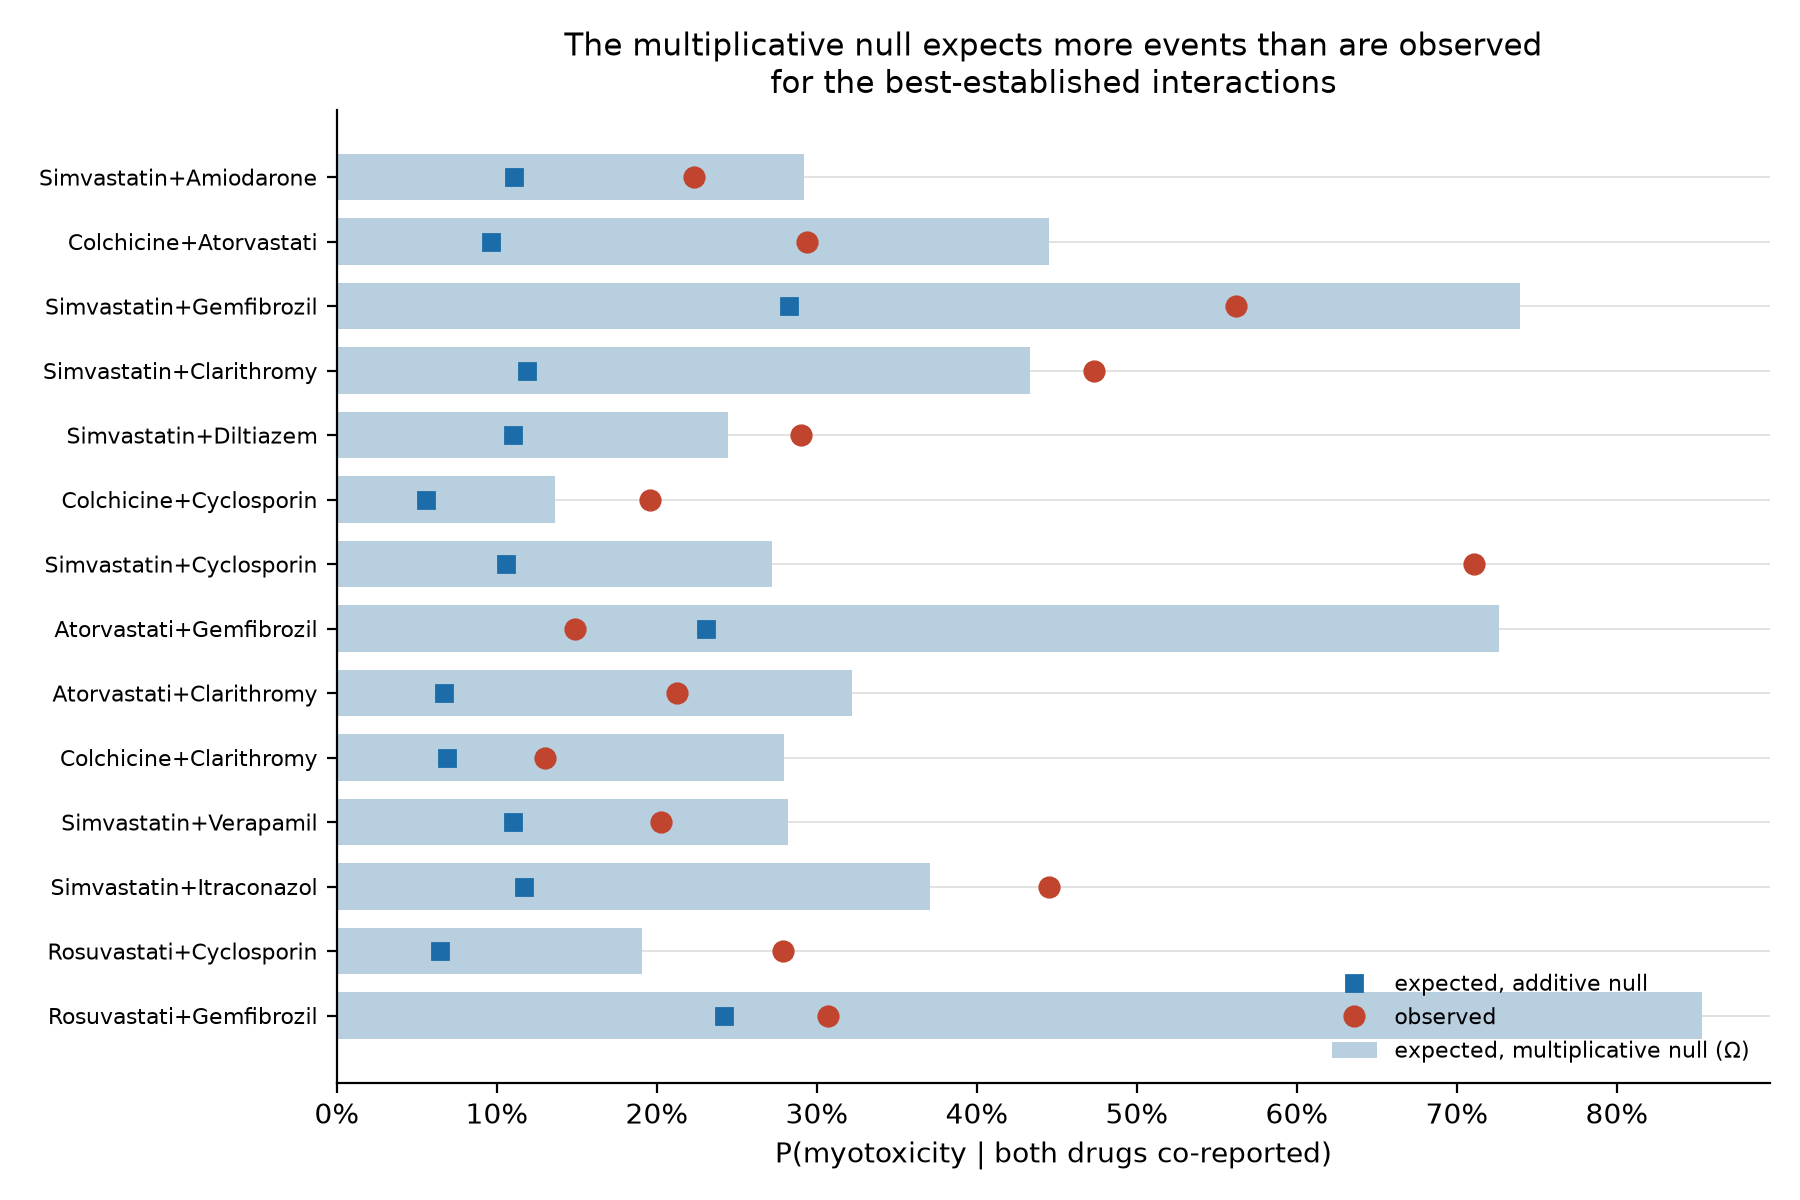
\includegraphics[width=0.85\linewidth]{figure1_null_comparison.png}
\caption{Observed proportion of co-reports carrying myotoxicity (red circles) against the proportion expected under the multiplicative null (bars) and the additive null (blue squares), for the 14 positive controls with ≥50 co-reports, ordered by co-report count. The multiplicative null expects more events than are observed for most established interactions, which is why Ω scores them as protective.}
\label{fig:1}
\end{figure}


\begin{figure}[htbp]
\centering
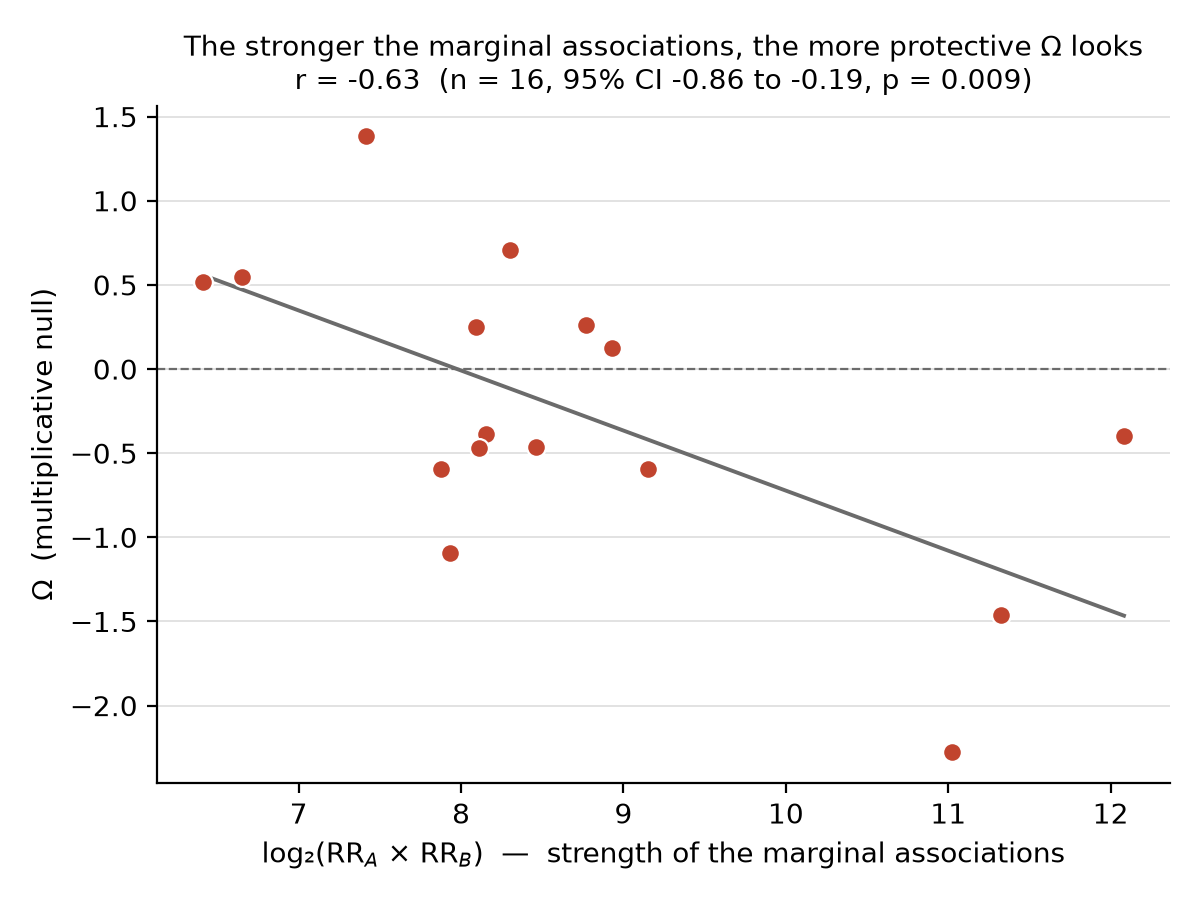
\includegraphics[width=0.85\linewidth]{figure2_omega_correlation.png}
\caption{Ω for each positive control against log₂(RR\_A × RR\_B), the combined strength of the two drugs' individual associations with the event. Line is ordinary least squares. The stronger the marginal associations, the more protective Ω appears.}
\label{fig:2}
\end{figure}


\begin{figure}[htbp]
\centering
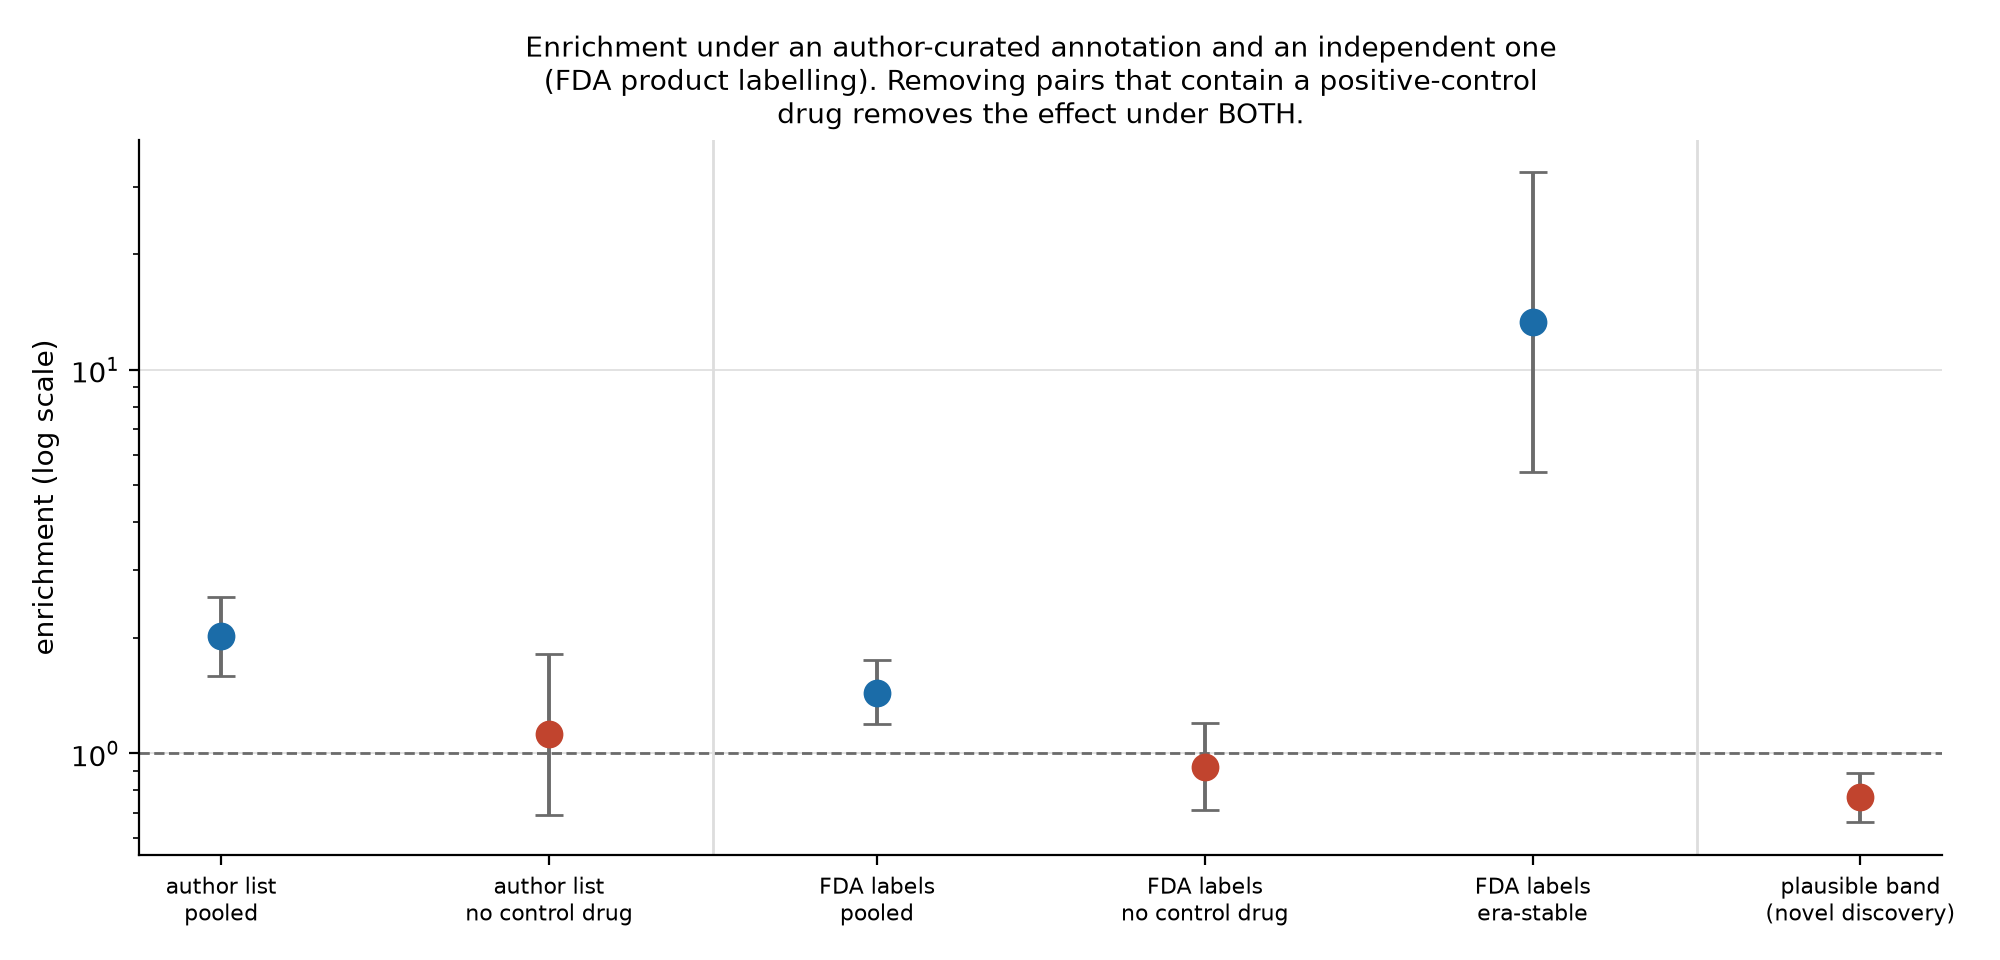
\includegraphics[width=0.85\linewidth]{figure3_band_enrichment.png}
\caption{Signal enrichment relative to unsupported pairs, log scale, with 95\% intervals. Five points in three groups. The first two are the author-curated annotation, pooled and then with pairs containing a positive-control drug removed; the middle two are the same contrast under the independent FDA-labelling annotation; the last is the plausible discovery band, the quantity those scopes are being compared against. Under both annotations, removing control-drug pairs moves enrichment to unity. The era-stable composition enrichment is deliberately \textbf{not} plotted here — it does not survive the two corrections applied to every other enrichment in this paper, and is tabulated with its corrections in §4.6.}
\label{fig:3}
\end{figure}


\begin{figure}[htbp]
\centering
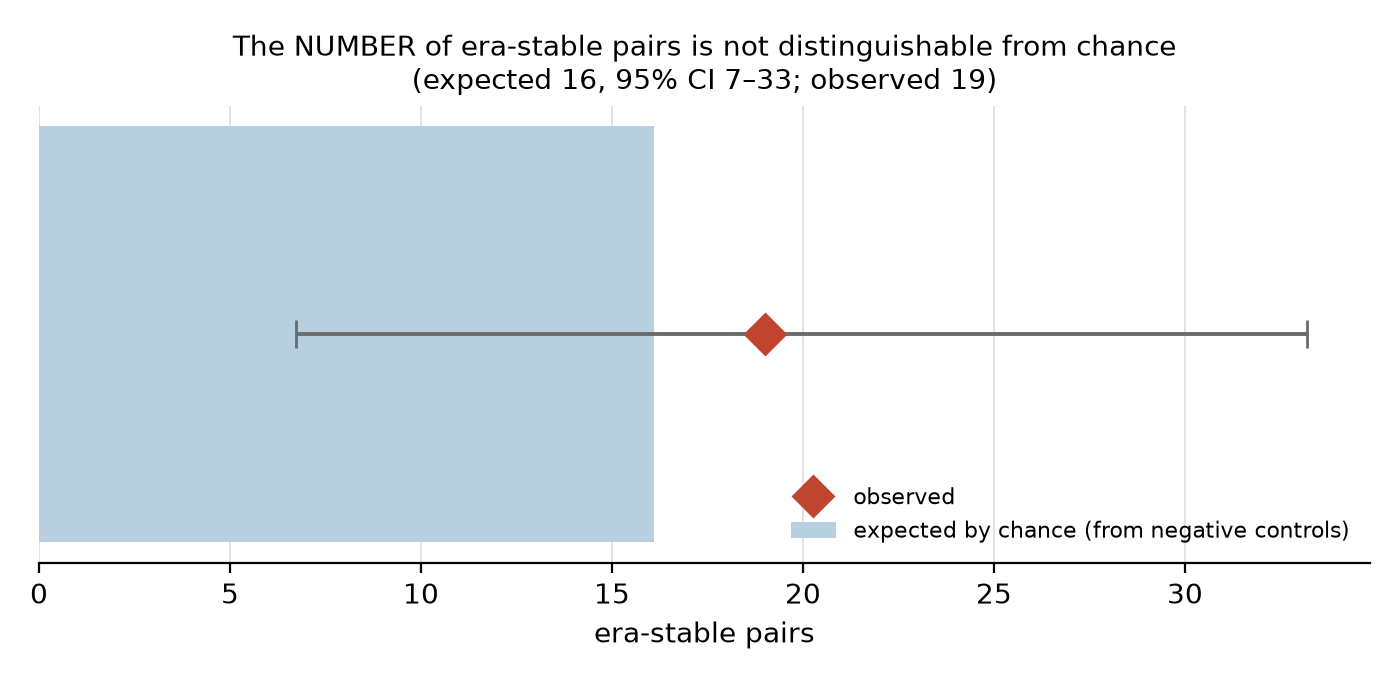
\includegraphics[width=0.85\linewidth]{figure4_era_stability.png}
\caption{Number of era-stable pairs observed (red diamond) against the number expected by chance (bar, with 95\% interval) computed by applying the same filter to the negative controls. The observed count lies inside the interval.}
\label{fig:4}
\end{figure}


\begin{figure}[htbp]
\centering
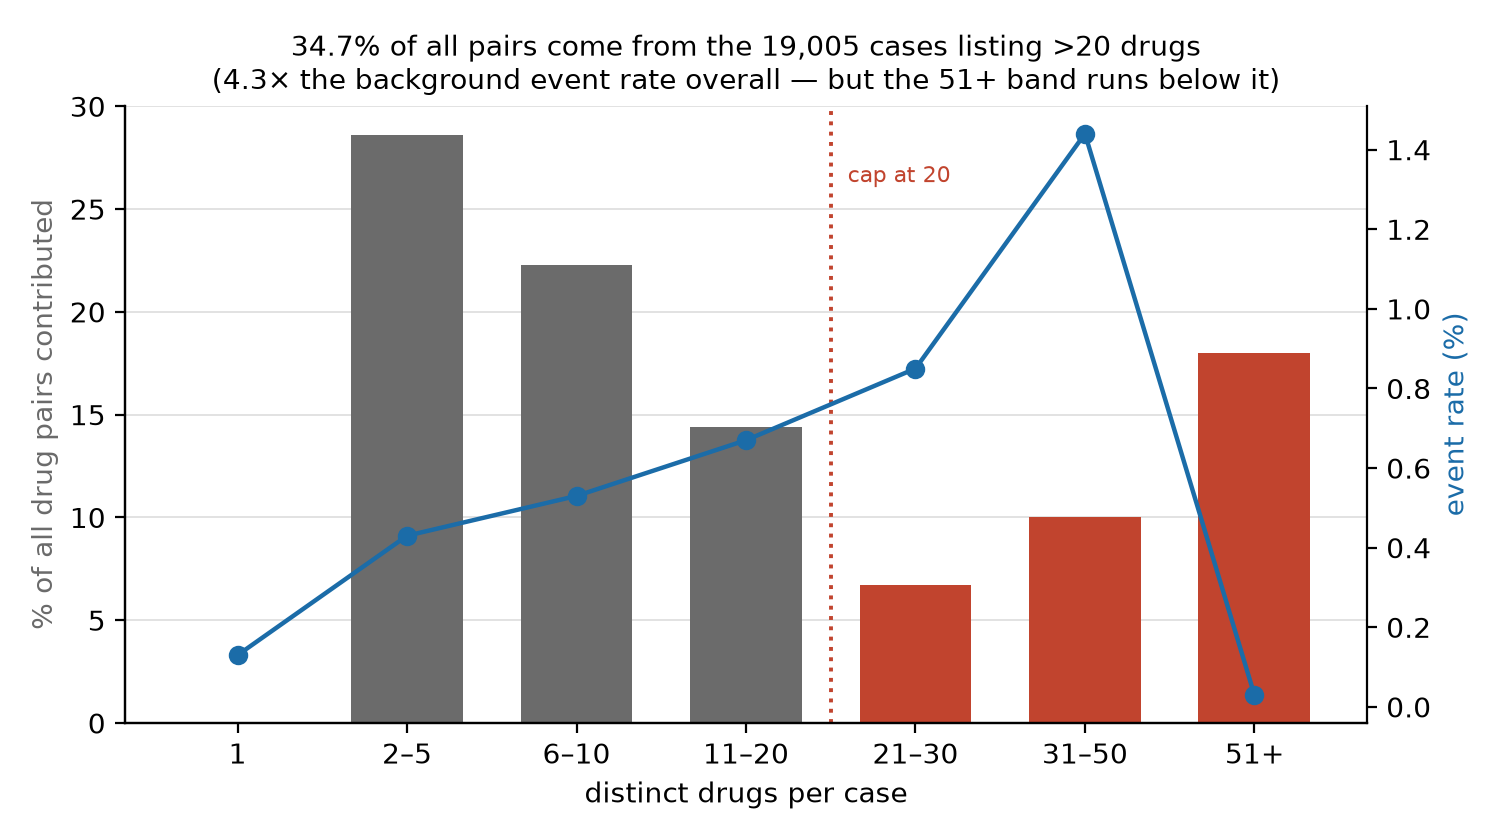
\includegraphics[width=0.85\linewidth]{figure5_polypharmacy_leverage.png}
\caption{Percentage of all drug pairs contributed by cases in each drugs-per-case band (bars, left axis) and the myotoxicity event rate within that band (line, right axis). Dotted line marks the cap adopted at 20 drugs.}
\label{fig:5}
\end{figure}


\begin{figure}[htbp]
\centering
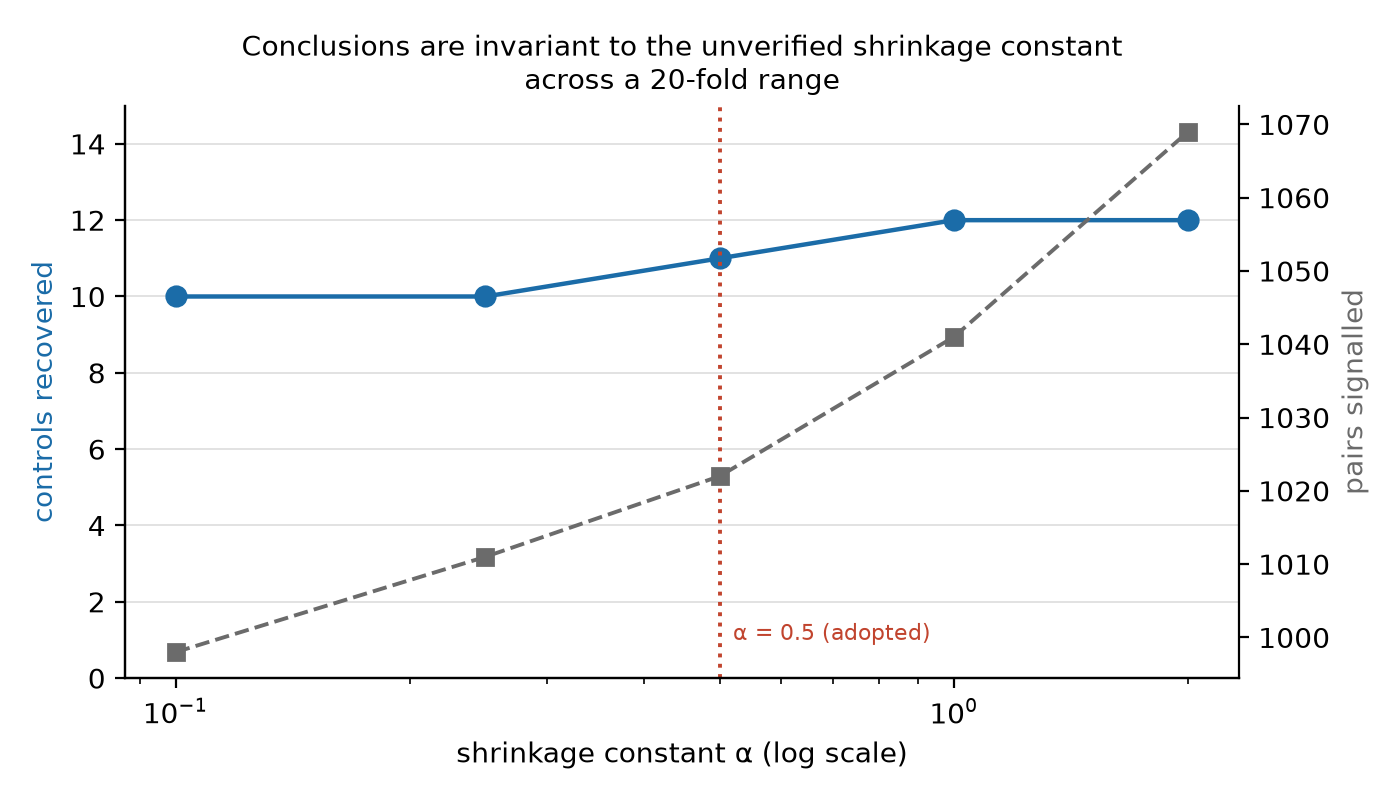
\includegraphics[width=0.85\linewidth]{figure6_alpha_sensitivity.png}
\caption{Positive controls recovered (left axis) and pairs signalled (right axis) as the shrinkage constant α varies over a 20-fold range, with the threshold recalibrated on the full negative pool at each value. Dotted line marks the adopted α = 0.5.}
\label{fig:6}
\end{figure}


\begin{figure}[htbp]
\centering
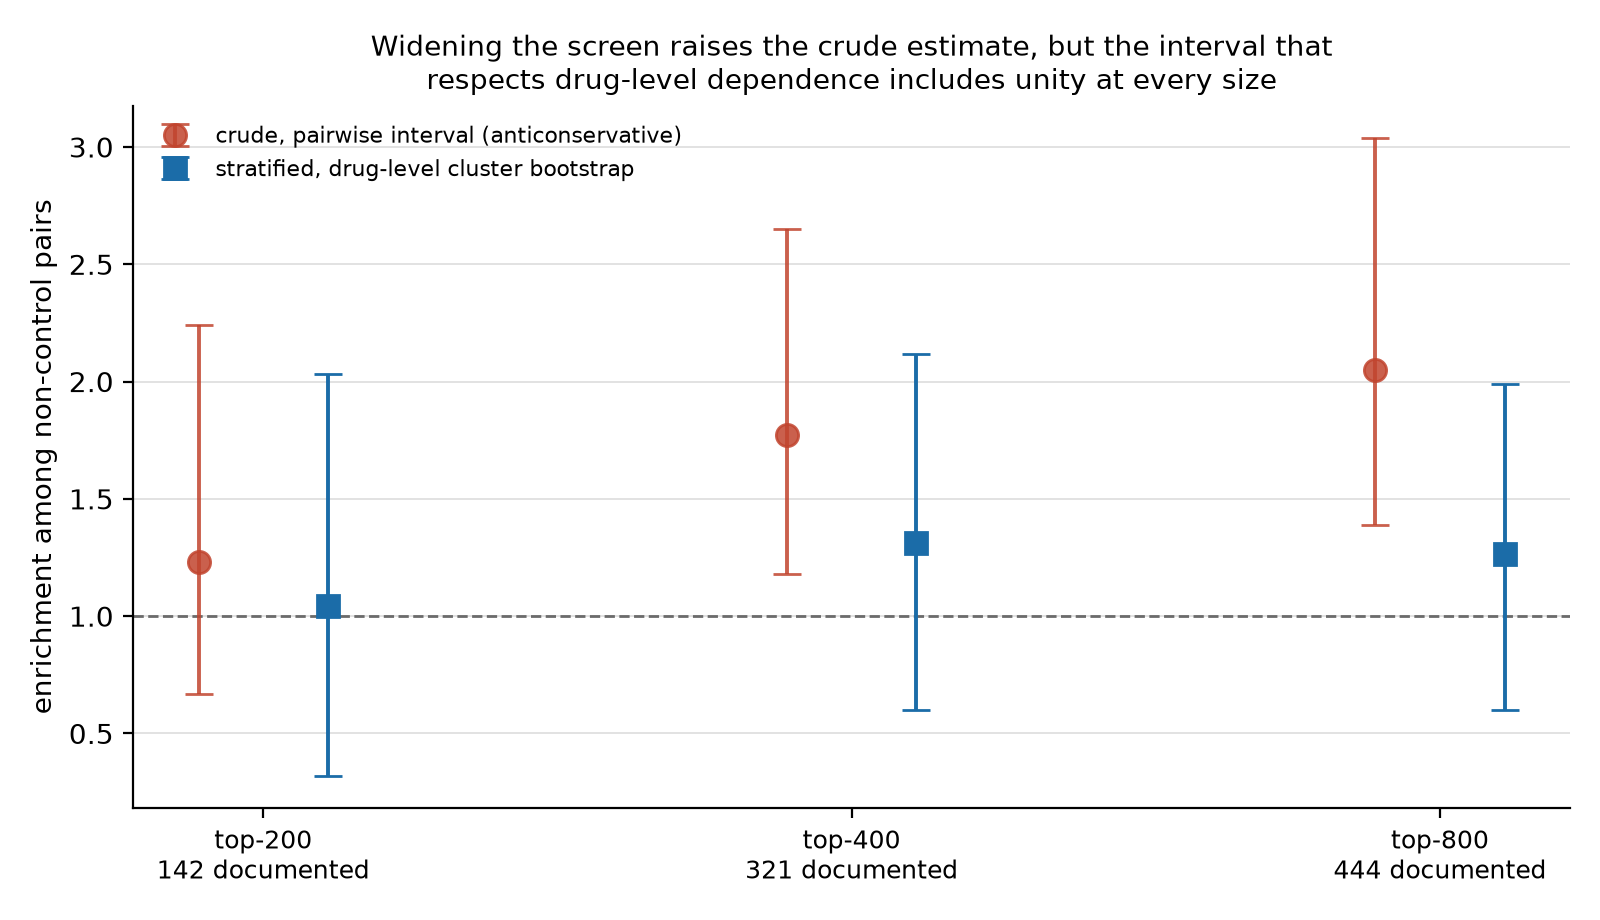
\includegraphics[width=0.85\linewidth]{figure7_screen_size_power.png}
\caption{Enrichment among non-control pairs at three screen sizes, under the pairwise interval (red, anticonservative because pairs share drugs) and the drug-level cluster bootstrap (blue). The cluster interval includes unity at every size.}
\label{fig:7}
\end{figure}

\end{document}
